\documentclass[conference]{IEEEtran}
\IEEEoverridecommandlockouts
% The preceding line is only needed to identify funding in the first footnote. If that is unneeded, please comment it out.
\usepackage{cite}
\usepackage{amsmath,amssymb,amsfonts}
\usepackage{algorithmic}
\usepackage{graphicx}
\usepackage{textcomp}
\usepackage{xcolor}
\usepackage{acronym}
\usepackage{listings}
\usepackage{setspace}
\usepackage{url}
\usepackage[utf8]{inputenc}
\def\BibTeX{{\rm B\kern-.05em{\sc i\kern-.025em b}\kern-.08em
    T\kern-.1667em\lower.7ex\hbox{E}\kern-.125emX}}
\begin{document}

\lstset{frame=tb,
	language=C,
	aboveskip=5mm,
	belowskip=5mm,
	showstringspaces=false,
	columns=flexible,
	basicstyle={\small\ttfamily},
	numbers=none,
	numberstyle=\tiny\color{gray},
	keywordstyle=\color{blue},
	commentstyle=\color{teal},
	stringstyle=\color{orange},
	breaklines=false,
	breakatwhitespace=false,
	tabsize=2,
	captionpos=b,
}
\lstset{language=C++}
\lstset{basicstyle=\scriptsize}
	
\newacro{CGRA}{Coarse-Grain Reconfigurable Array}
\newacro{CPU}{Central Processing Unit}
\newacro{ISA}{Instruction Set Architecture}
\newacro{UART}{Universal Asynchronous Receiver-Transmitter}
\newacro{LED}{Light Emitting Diode}
\newacro{CM}{Configuration Module}
\newacro{DE}{Data Engine}
\newacro{FU}{Functional Units}
\newacro{AGU}{Address Generation Unit}
\newacro{LUT}{Lookup Tables}
\newacro{FPGA}{Field-Programmable Gate Array}
\newacro{ASIC}{Application-Specific Integrated Circuit}
\newacro{CPI}{Cycles Per Instruction}
\newacro{CNN}{Convolutional Neural Network}
\newacro{HDL}{Hardware Description Language}
\newacro{RTL}{Register-Transfer Level}
\newacro{UUT}{Unit Under Test}
\newacro{VPI}{Verilog Procedural Interface}
\newacro{API}{Application Programming Interface}
\newacro{DMA}{Direct Memory Access}
\newacro{VCD}{Value Change Dump}
\newacro{BRAM}{Block Random Access Memories}
\newacro{DSP}{Digital Signal Processor}
\newacro{ASIP}{Application Specific Instruction Set Processors}
\newacro{ALU}{Arithmetic Logic Unit}


\title{Deep Neural Networks on the Versat Reconfigurable Processor\\ }

\author{\IEEEauthorblockN{João Pedro Costa Luís Cardoso}
\IEEEauthorblockA{\textit{Electrical and Computer Engineering Department} \\
\textit{Instituto Superior Técnico}\\
Lisbon, Portugal \\
joao.pedro.cardoso@tecnico.ulisboa.pt}
}

\maketitle

\begin{abstract}
This paper presents the problem of accelerating the execution of Deep Neural
Networks (DNNs) using Coarse-Grained Reconfigurable Arrays (CGRAs), 
with special emphasis on compiling a DNN description into code that runs on a
CPU/CGRA system. This topic is a vast one, so this paper focuses on simulating
DeepVersat , a CPU/CGRA system suitable for DNN, and tools for running any
Convolutional Neural Network on DeepVersat. The tools presented in this paper
allow for architectural exploration and optimization, and a dramatic reduction
of the development time.
\end{abstract}

\begin{IEEEkeywords}
CGRA, Versat, Darknet, Convolutional Neural Networks, Deep Neural Networks
\end{IEEEkeywords}

%%%%%%%%%%%%%%%%%%%%%%%%%%%%%%%%%%%%%%%%%%%%%%%%%%%%%%%%%%%%%%%%%%%%%%%%%%%%%%%%%%%%%%%%%%

\section{Introduction}
\IEEEPARstart{N}{e}ural Networks have been an object of study since the 1940s but until the
beginning of this decade their applications were limited and did not play a
major role in computer vision conferences. With its meteoric rise in research,
several solutions to accelerate this algorithm have appeared, from Field Programmable Gate Arrays (FPGA) to
Application Specific Integrated Circuits (ASIC) implementations.

Convolutional Neural Networks (CNNs) are a particular kind of DNN where the output
values of the neurons in one layer are convolved with a kernel to produce the
input values of the neurons of the next layer. This algorithm is compute bound,
that is, its performance depends on how fast it can do certain calculations, and
depend less on the memory access time. Namely, the convolutional layers take
approximately 90$\%$ of the computation time.

The acceleration of these workloads is a matter of importance for today's
applications such as image processing for object recognition or simply to
enhance certain images. Other uses like instant translation and virtual
assistants are applications of neural networks and their acceleration is of
vital importance to bring them into the Internet of Things.

A suitable circuit to accelerate DNNs in hardware is the CGRA. A CGRA is a
collection of Functional Units and memories with programmable interconnections
to form computational datapaths. A CGRA can be implemented in both
FPGAs and ASICs. CGRAs can be reconfigured much faster than FPGAs, as they have
much fewer configuration bits. If reconfiguration is done at runtime, CGRAs add
temporal scalability to the spacial scalability that characterizes
FPGAs. Moreover, partial reconfiguration is much easier to do in CGRAs compared
to FPGAs which further speeds up reconfiguration time. Another advantage of
CGRAs are the fact that they can be programmed entirely in software, contrasting
with the large development time of customized Intellectual Property (IP) blocks.
The Coarse Grain Reconfigurable Array (CGRA) is a midway acceleration solution
between FPGAs, which are flexible but large, power-hungry, and difficult to
reprogram, and ASICs, which are fast but generally not programmable.

However, mapping a specific DNN to a CGRA requires knowledge of its
architecture, latencies, and register configurations, which may become a lengthy
process, especially if the user wants to explore the design space for several
DNN configurations. An automatic compiler that can map a standard DNN
description into CPU/CGRA code would dramatically decrease the time to market of its
users. Currently, there are equivalent tools for CPUs and GPUs and
even for FPGAs.

The DeepVersat CGRA is the DNN accelerator to improve the performance of the DNNs in embedded hardware.
Another objective is to increase the versatility of the Versat API and offer new functions
to simplify the development of new software. One of these functions is a generic convolution for
Versat which can, independently of the hardware configuration, configure the convolution to have
the highest performance possible on the available functional units while being dynamic and
to avoid developer work to adapt to new convolutions.

%%%%%%%%%%%%%%%%%%%%%%%%%%%%%%%%%%%%%%%%%%%%%%%%%%%%%%%%%%%%%%%%%%%%%%%%%%%%%%%%%%%%%%%%%%

\section{Deep Neural Networks}
\label{chapter:cnn}

\begin{figure}[!htb]
    \centering
    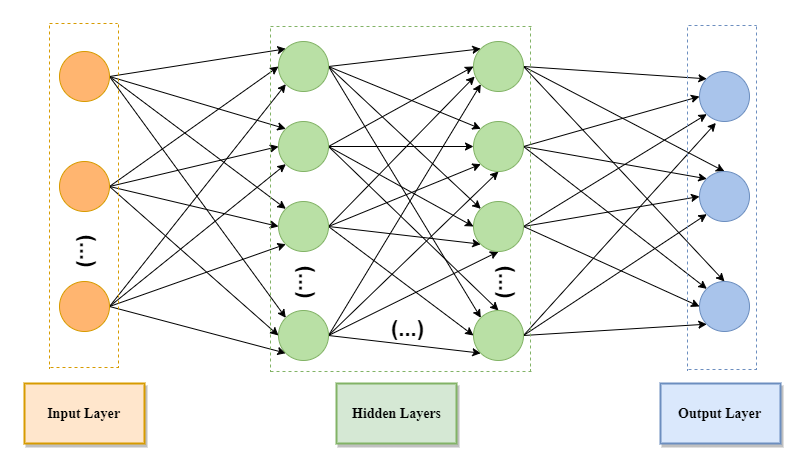
\includegraphics[width=0.4\textwidth]{Figures/mlp.png}
    \caption{Deep Neural Network Structure}
    \label{MLP}
\end{figure}

A Neural Network (NN) is an interconnected group of nodes that follow a
computational model that propagates data forward while processing. The earliest
NNs were proposed by McCulloh and Pitts~\cite{neuron:model}, in which a neuron
has a linear part, based on an aggregation of data and then a non-linear part
called the activation function, which is applied to the aggregate sum. The issue
with using only one neuron is that it is not able to be used in non-linear
separable problems. By aggregating several neurons in layers and the input of
each neuron as in figure~\ref{MLP} being based on the previous layers, that
problem can be eliminated.

Each input to a neuron contributes differently to the output. The share is
dependent on the weight value. These are obtained by training the network
through various techniques, one of which is called Deep Supervised
Learning~\cite{deeplearning} . For a certain input, there is an expected output
and the real output of the NN. Then the loss function (the difference) is
calculated and the weight values are iteratively modified for improving the
outputs of the NN.

A Deep Neural Network (DNN) is a Neural Network that uses this approach for
learning. It has multiple hidden layers and it can model complex non-linear
relationships. If the activation function is non-polynomial, it satisfies the
Universal approximation problem~\cite{approximation:problem}.

One of the limitations of traditional NNs is the complexity of layer
interconnections. Using as an example the hand digit recognition problem and MNIST
data set, composed of 28x28 grayscaled images~\cite{mnist:digits}, in a
traditional fully connected NN, a neuron from the second layer would have 28x28
weights. That is 3.136 kiloBytes per neuron of weight values while using 32-bit
floating-point numbers (FP32). When building a more complex network for image
recognition, the computational complexity grows quadratically with the number
of neurons per layer.


\subsection{Convolutional Neural Networks}
\label{section:cnn}

 \begin{figure}[!htb]
    \centering
    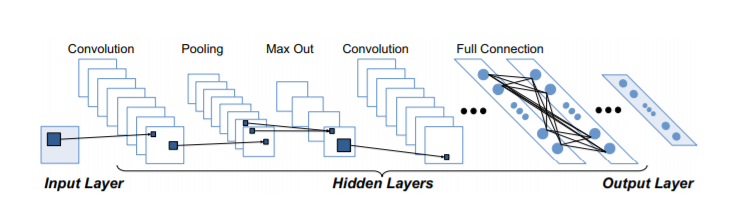
\includegraphics[width=0.4\textwidth]{Figures/convolutionlayer.png}
    \caption{CNN architecture example, taken from~\cite{cgracnn}}
    \label{CNNl}
\end{figure} 

Convolutional Neural Networks (CNN) are a class of DNNs used in Image and Video
recognition due to their shift invariance characteristic. They were first
proposed in the 1980s but it was not until 2012 with AlexNet~\cite{alexnet} that
CNNs took off. Fundamentally, CNNs are a regularized version of
Multilayer Perceptrons (MLP). These networks fix the complexity issue discussed
as each neuron is only connected to a few neurons of the previous layer.


\paragraph{Convolutional Layer}
\label{section:convlayer}

In a typical CNN, not all layers are convolutional, but the convolutional layers
are the most compute-intensive ones. CNNs take input images with three  dimensions
(width, height, and color space); for the following convolutional layers 3D
arrays are used (width, height, and number of channels). For the earlier example
of the MNIST data set, the input would have dimensions 28x28x1 as it is a 2D
image in grayscale.

To compute a neuron in the next layer we use the convolution
equation~\ref{equation:convolution} aided by Figure~\ref{Cl}.
\begin{equation} \label{equation:convolution}
   %\resizebox{.5 \textwidth}{!} 
    %%
\end{equation}
where $x_{j}^{l+1}$ is the output, $\delta$ is the activation function, which
depends on the architecture, $x_{i}^{l}$ is the input of the convolution layer,
$k_{ij}^{l+1}$ is the kernel of the said layer which is obtained by training the
network, and $b_{j}^{l+1}$ is the bias.

Thus an output neuron depends only on a small region of the input which is
called the local receptive field.

\begin{figure}[!htb]
    \centering
    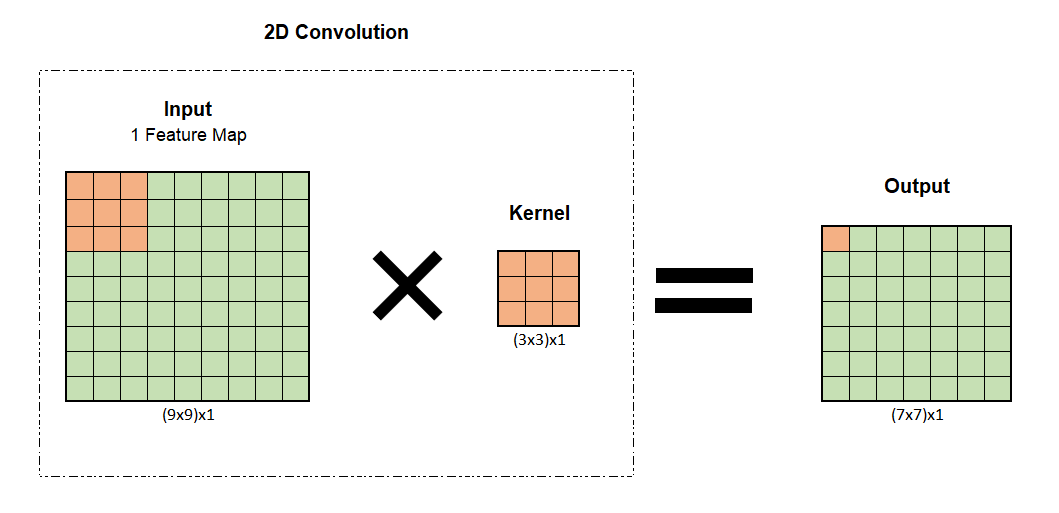
\includegraphics[width=0.4\textwidth]{Figures/conv.png}
    \caption{2D convolution with stride = one and without zero padding}
    \label{Cl}
\end{figure} 


The output's dimensions depend on several parameters of the convolution such as
zero-padding and stride. The former means to add zeros around the edges of the
input matrix. The latter means the step used for the convolution, if the value
is e.g. 2, it will skip a pixel each iteration of the convolution.
Equation~\ref{equation:padding} can be used to calculate the output size.

\begin{equation} \label{equation:padding}
     n^{l+1} = \frac{n^{l}- b^{l}+2 \times p}{s} + 1
\end{equation}
where $n$ is the width/height of the input of layer $l$, $ b$ is the
width/height of the kernel, $p$ is zero-padding while $s$ is the stride.

The number of channels of the output is equal to the number of filters in the
convolutional layer.

%Then a 3D convolution is performed with the kernel changing from layer to layer

\paragraph{Pooling Layer}

The MaxPool or AvgPool are layers used in Convolutional Neural Networks to
downsampling the feature maps to make the output maps less sensitive to the
location of the features.

Maximum Pooling or MaxPool, like is suggested in its name groups $ n * n $
points and outputs the pixel with the highest value.  The output will have its size
lowered by $n$ times.  The Average Pooling or AvgPool, instead takes all of
the input points and calculates the average. Downsampling can also be achieved
by using convolutions with stride two and padding equal to 1.  Upsample layers can
be also used that turn each pixel into $n^{2}$, where $n$ is the number of times
the output will be bigger than the input.

% \begin{figure}[!htb]
%     \centering
%     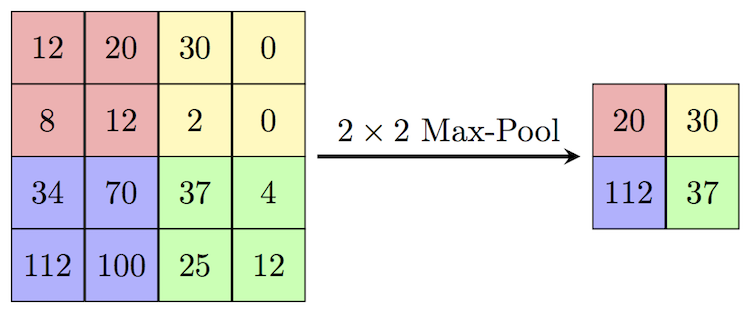
\includegraphics[width=0.4\textwidth]{Figures/maxpool.png}
%     \caption{Simple example of a max pool layer~\cite{maxpoolimg}}
%     \label{figure:maxpool}
% \end{figure} 
 

\paragraph{Fully Connected Layer}

The fully connected layer is mostly used for classification in the final layers
of the NN. It associates the feature map with the respective labels.  It takes the
3D vector and outputs a single vector thus it is also known as flatten.
Equation~\ref{equation:connected} describes the operation.

\begin{equation} \label{equation:connected}
    %\resizebox{.5 \textwidth}{!} 
     %%
\end{equation}
where $w_{ji}^{l+1}$ are the weights associated with a specific input for each output.


\paragraph{Route $\&$ Shortcut Layer}

The Shortcut layer or skip connection was first introduced in
Resnet~\cite{resnet}.  It allows connecting of the previous layer to another to
allow the flow of information across layers.  The Route layer, used in
Yolov3~\cite{yolov3}, concatenates two layers in depth (channel) or skips the
layer forward. This is used after the detection layer in Yolov3 to extract other
features.

\paragraph{Dropout Layer}

This type of layer was conceived to avoid overfitting~\cite{Dropout} by dropping
the neurons with a probability below the threshold. 
% In Figure~\ref{figure:Dropout}, there is a graphical representation.
% \begin{figure}[!htbp]
%     \centering
%     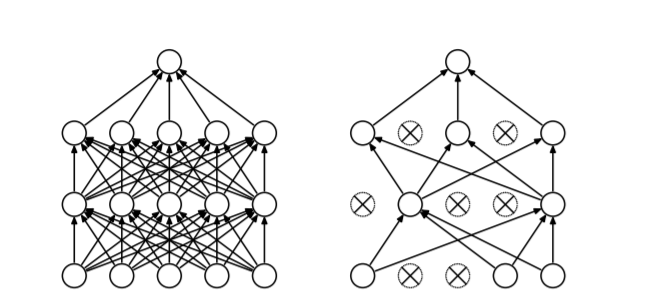
\includegraphics[width=0.4\textwidth]{Figures/dropout.png}
%     \caption{Dropout if applied to all layers, adapted from~\cite{Dropout}}
%     \label{figure:Dropout}
% \end{figure} 

\paragraph{Activation Functions}

Activation Functions (AF) are functions used in each layer of a NN
to compute the weighted sum of input and biases, which is used to give a value
to a neuron. Non-linear AFs are used to transform linear inputs into non-linear
outputs.  While training Deep Neural Networks, vanishing and exploding
gradients are common issues, in other words, after successive multiplications
of the loss gradient, the values tend to 0 or infinity and thus the
gradient disappears. AFs help mitigate this issue by keeping the gradient within
specific limits. The most popular activation functions can be found in
table~\ref{table:AF}.

% \begin{table}[htb]
%     \centering
%     \resizebox{1\textwidth}{!}{%}
%     \begin{tabular}{ll}
%     \hline
%     \textbf{Activation Functions} & \textbf{Computation Equation} \\ \hline \hline
%     Sigmoid                       &  $\displaystyle f(x)=\frac{1}{1+ e^{-x}}$                             \\ \hline
%     Tanh                          &  $\displaystyle f(x)=\frac{e^{x}-e^{-x}}{e^{x}+e^{-x}}$                            \\ \hline
%     Softmax                       &  $\displaystyle f(x_{i})=\frac{x_{i}}{\sum_{j}e^{x_{j}}}$                             \\ \hline
%     ReLU                          &    $ f(x)=\begin{matrix}
%         x & if & x\geq 0  \\ 
%         0 & if & x< 0 
%     \end{matrix} $                           \\ \hline
%     LReLU                         &  $f(x)= \begin{matrix}
%         x & if & x > 0  \\ 
%         \alpha x & if & x \leq 0 
%     \end{matrix} $                        \\ \hline
%     ELU                           &             $ f(x)=\begin{matrix}
%         x & if & x> 0  \\ 
%         \alpha e^{x} - 1 & if & x\leq 0 
%     \end{matrix} $                 \\ \hline
%     \end{tabular}%
%     }
%     \caption{Popular activation functions}
%     \label{table:AF}
% \end{table}

\begin{table}[htb]
    \centering
    \resizebox{0.4\textwidth}{!}{%
    \begin{tabular}{|l|l|}
    \hline
    \textbf{Activation Functions} & \textbf{Computation Equation} \\ \hline
    Sigmoid                       &  $f(x) = \dfrac{1}{1 + e^{-x}}$                             \\ \hline 
    Tanh                          &  $f(x) = \dfrac{e^{x} - e^{-x}}{e^{x} + e^{-x}}$                            \\ \hline
    Softmax                       &  $f(x_{i}) = \dfrac{x_{i}}{\sum_{j}e^{x_{j}}}$                             \\  \hline 
    ReLU                          &  $f(x) = \begin{cases} x & \text{if } x \geq 0 \\ 0 & \text{if } x < 0 \end{cases}$                           \\ \hline 
    LReLU                         &  $f(x) = \begin{cases} x & \text{if } x > 0 \\ \alpha x & \text{if } x \leq 0 \end{cases}$                        \\ \hline 
    ELU                           &  $f(x) = \begin{cases} x & \text{if } x > 0 \\ \alpha e^{x} - 1 & \text{if } x \leq 0 \end{cases}$                 \\ \hline
    \end{tabular}%
    }
    \linebreak
    \caption{Popular activation functions}
    \label{table:AF}
	\vspace{\abovecaptionskip}
\end{table}


%image of activation functions?

 \subsection{Frameworks for Neural Networks}
 \label{section:Darknet}

To run a Neural Network model there are several popular frameworks like
Tensorflow, PyTorch, Caffe, and Darknet.  Their purpose is to offer abstraction
to software developers that want to run these networks. They also offer
programming for different platforms like Nvidia GPUs by using the CUDA API.

\subsubsection{Darknet}

Darknet~\cite{Darknet} is an open-source neural network framework written in C
and CUDA. It is used as the backbone for Yolov3~\cite{yolov3} and supports
several different network configurations such as AlexNet and Resnet.  It
utilizes a network configuration file (.cfg) and a weights file (.weights) as
input for inference.

\begin{figure}[!htb]
\lstinputlisting[label=cfg,language=Python,frame=single,breaklines=true,firstline=13,lastline=19,caption=cfg
  code for a Convolutional Layer used in
  Yolov3~\cite{yolov3}]{./Code/yolov3.cfg}
\end{figure}

In Listing~\ref{cfg}, there is a snippet of the file featuring a convolution
layer with 32 kernels of size 3x3. It has stride one and zero padding of 1,
meaning the output size equals the input size. The input size can be
calculated by analyzing the previous layers and the network parameters. The
network parameters includes data to be used for training while only
the first three parameters are needed for inference.

% \lstinputlisting[label=net,language=Python,frame=single,breaklines=true,firstline=1,lastline=11,caption=cfg
%   code for the network parameters]{./Code/yolov3.cfg}


\subsubsection{Caffe}

Convolutional Architecture for Fast Feature Embedding (Caffe)~\cite{caffe} is
also an open-source framework written in C++ with a Python interface.  Caffe
exports a neural network by serializing it using the Google Protocol Buffers
(ProtoBuf) serialization library. Each network has two prototxt files:
\begin{itemize}
    \item deploy.prototxt- File that describes the structure of the network that
      can be deployed for inference.
    \item train\_val.prototxt- File that includes structure for training.  it
      includes the extra layers used to aid the training and validation process.
\end{itemize}

The Python interface helps generate these files. For inference only the
deploy file matters. 
% In Listing~\ref{caffe}, there is a snippet of a deployed file. 

% \lstinputlisting[label=caffe,language=Python,frame=single,breaklines=true,firstline=1,lastline=26,caption=prototxt
%   file for the input data and the first convolution layer of
%   AlexNet~\cite{alexnet}]{./Code/caffe.prototxt}



%%%%%%%%%%%%%%%%%%%%%%%%%%%%%%%%%%%%%%%%%%%%%%%%%%%%%%%%%%%%%%%%%%%%%%%%%%%%%%%%%%%%%%%%%%





\section{DeepVersat}
\label{sector:DeepVersat}

\quad Versat is a Coarse-Grained Reconfigurable Array (CGRA) Architecture. CGRAs are in-between Field Programmable Gate Arrays (FPGA)
 and general purpose processors (GPP).
The former is fully reconfigurable and the highest performance for a workload can be achieved as the Architecture is tailored to the workload.
GPPs on the other hand, are not reconfigurable and thus slower but are more generic and can process different workloads.
While FPGAs have granularity at the gate level, CGRAs have granularity at the functional unit level. They are configurable at run-time and the datapath can be
changed in-between runs.

\subsection{Versat Architecture}

\quad The Versat Architecture~\cite{sousa:compiler,sousa:controller,sousa:FFT,sousa:versat2016} 
is depicted in Figure~\ref{figure:oldversat}. It is composed of the following modules: DMA, Controller, Program Memory, Control File Registry, Data Engine, and Configuration module.
The Controller accesses the modules through the control bus. The code made in assembly or C is loaded into the program Memory (RAM) where the user
can write to the configuration module for the Versat runs. Between runs of the Data Engine,
 the Controller can start doing the next run configuration and calculations.


\begin{figure}[!htbp]
    \centering
    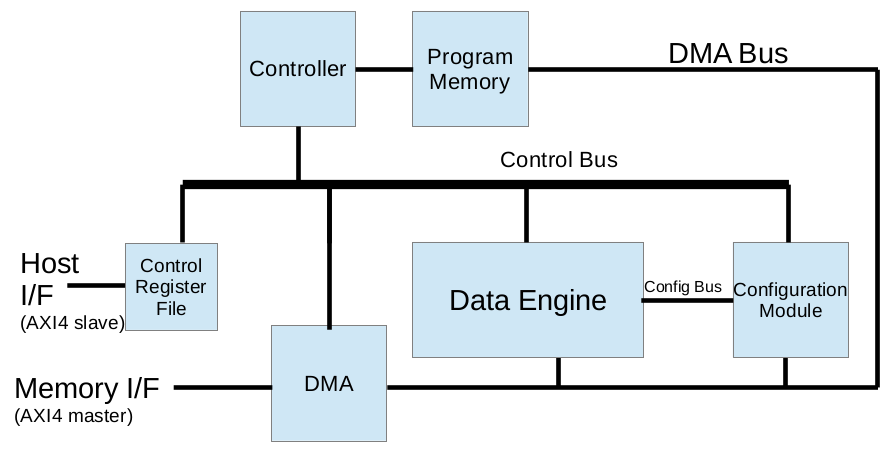
\includegraphics[width=0.4\textwidth]{Figures/top.png}
    \caption{Versat Topology~\cite{sousa:controller}}
    \label{figure:oldversat}
\end{figure} 

\subsubsection{Data Engine}
% \begin{figure}[!htbp]
%     \centering
%     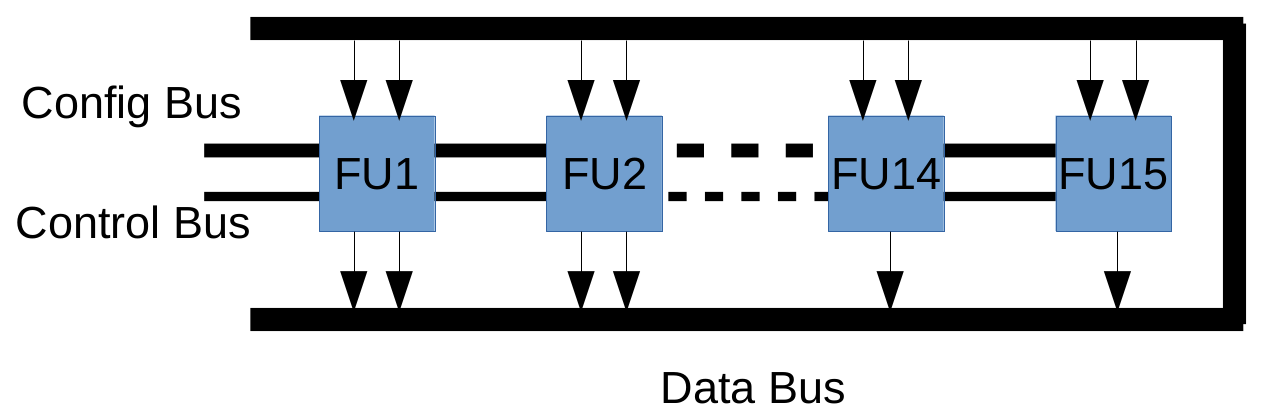
\includegraphics[width=0.4\textwidth]{Figures/de.png}
%     \caption{Versat Data Engine Topology~\cite{sousa:FFT}}
%     \label{figure:DE}
% \end{figure} 


The Data Engine carries out the computation needed on the data arrays. It is a 32-bit architecture with up to 11 Functional Units (FU):
 Arithmetic and Logic Unit(ALU), stripped down ALU (ALU-Lite),
 Multiplier and Accumulator (MAC) and Barrel Shifter.
 Depending on the project and calculations, a new type of FU or the existing ones can be altered to support the algorithm.
 The DE has a full mesh topology, which means that each FU can be the output to another, which leads to a decrease in operating frequency.

 Each Input of a Functional Unit has a Mux with 19 entries, eight of which are from the memories (2 from each Mem out of four total units) and the rest from the Functional Units (11).

 \begin{figure}[!htbp]
    \centering
    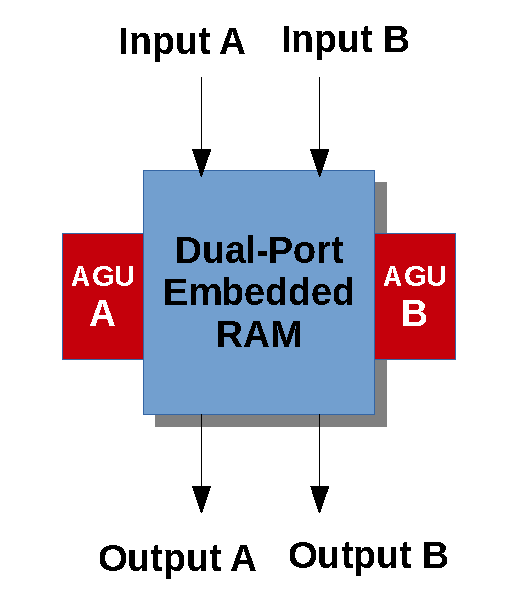
\includegraphics[width=0.2\textwidth]{Figures/fu2.pdf}
    \caption{Versat Memory Unit with one AGU per port~\cite{lopes:Versat}}
    \label{figure:FU}
\end{figure} 


 The four Memories are dual port and for the input of both ports, 
 there is an Address Generation Unit (AGU) that is able to 
 reproduce two nested loops of memory indexes.
 The AGUs control which MEM data is the input of the FUs and where
 to store the results of the operation. Also, the AGUs support delayed start to line up timings
due to latencies. The memory module is represented in Fig~\ref{figure:FU}.

\subsubsection{Configuration Module}
Versat has several configuration spaces devised for each Functional Unit,
with each space having multiple fields to define the operation of the Functional unit (e.g. which op for the ALU).
These are accessed before the run by the controller to define the datapath.

% \begin{figure}[!htbp]
%     \centering
%     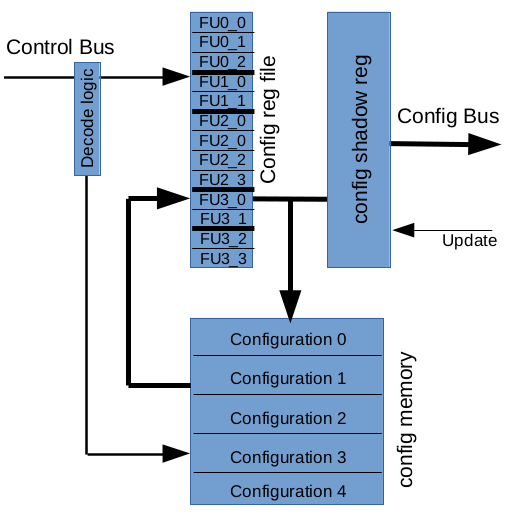
\includegraphics[width=0.25\textwidth]{Figures/conf.png}
%     \caption{Configuration Module~\cite{sousa:controller}}
%     \label{figure:conf}
% \end{figure} 

The Configuration Module (CM), 
has three components: configuration memory, variable length configuration register file 
and configuration shadow register.
The latter holds the current configuration so the controller can change the values of the configuration file in-between runs.
The decode logic finds which component to write or read, if it's the registers, it ignores read operations.
Meanwhile, the configuration memory interprets both write and reads. When it receives a read,
it writes into the register configuration data, when it's a write, it stores the data instead.


\subsection{DeepVersat Architecture}
\label{subsection:deepversat1}

\begin{figure}[!htb]
    \centering
    \includegraphics[width=0.4\textwidth]{Figures/deep-Versat.png}
    \caption{DeepVersat Architecture~\cite{valter:deepversat}}
    \label{figure:deepversatarch}
\end{figure} 

\quad The DeepVersat Architecture~\cite{valter:deepversat}
, in figure~\ref{figure:deepversatarch}, decouples the Data Engine (DE) from all control and as such, it can be used with any CPU. 
It can be paired with hard cores in
FPGA boards like the ZYNC board %cite here
with its A9 ARM dual-core CPUs or pair it with a soft core.

Its principle is to create the concept of a Versat Core: Configuration Module (CM) and its Functional Units (FU) connected with a control bus and a data bus.
Instead of writing to memory, there is the option to write for the next
Versat Core to create more complex and more complete Datapaths, to avoid
having to reconfigure the cores.

The number of Layers and FUs are reconfigurable pre-silicon with the only limitation
that each layer is identical. To program DeepVersat, an API is generated
from the Verilog .vh files. 




\subsubsection{DeepVersat System}

\begin{figure}[!htbp]
    \centering
    \includegraphics[width=0.4\textwidth]{Figures/deep-Versat-top.png}
    \caption{DeepVersat System using a RISC-V RV32IMC soft processor~\cite{valter:deepversat}}
    \label{figure:deepversattop}
\end{figure} 

\quad To make a complete system, a new controller is needed with a more robust toolchain.
In a recent dissertation~\cite{valter:deepversat}, the IOB-RV32 processor was used which uses the RISC-V Instruction Set (ISA) with 32-bit Integer base alongside Multiplication and Division extension and Compact Instruction extension.
 The core is derived from
the open-source PicoRV32 CPU~\cite{picorv}.
The IOB-RV32 uses its memory bus to access peripherals in which DeepVersat and the UART module are connected as such.
The control bus is used to access the configuration modules of DeepVersat. The data bus is used to read and write
a large amount of data into DeepVersat. The data flow bus is reserved for inter-Versat Core communication.

% \begin{table}[!htbp]
%     \centering
%     \begin{tabular}{|l|l|}
%         \hline
%         \textbf{Peripheral}     & \textbf{Memory address} \\ \hline
%         UART module             & 12’h100xxxxx            \\ \hline
%         DeepVersat control bus & 8’h11xxxxxx             \\ \hline
%         DeepVersat data bus    & 8’h12xxxxxx             \\ \hline
%         \end{tabular}
%     \linebreak
%     \caption{DeepVersat Memory Map}
%     \label{table:deepversat}
%     \end{table}


To address the peripherals, each Versat has 15 bits of address while the CPU addresses
 the peripherals with 32 bits, with eight of those occupied to choose
 the peripheral in question. That leaves nine bits to address several Versat Cores
 which brings the theoretical maximum Versat cores to 512. The IOB-RV32 is compatible with the
 GNU toolchain to offer better portability of code and alongside the C++ Versat API the difficulty
 to code for the System diminishes.

%%%%%%%%%%%%%%%%%%%%%%%%%%%%%%%%% CNN VERSAT %%%%%%%%%%%%%%%%%%%%%%%%%%%%%%%%%%%%%%%%%%%%%%%%%%%%

\section{CNN Compiling in FPGAs}
\label{section:CNNVersat}

%PAPERS
%https://www.cv-foundation.org/openaccess/content_cvpr_workshops_2014/W17/html/Gokhale_A_240_G-opss_2014_CVPR_paper.html
%

\subsection{Toolflows for Mapping CNNs in FPGAs}
\label{section:toolflow}

Several software frameworks have been developed to accelerate the development and
execution of CNNs. The neural networks frameworks discussed in
section~\ref{section:Darknet} provides high-level APIs together with high-performance 
execution on multi-core CPUs, GPUs, Digital Signal Processors (DSPs)
and Neural Processing Units (NPUs)~\cite{smartphones}. FPGAs provide an
alternative to these architectures as they provide high performance while also
being low-power. FPGAs can meet several requirements including throughput and latency
in the diversity of applications. Thus, several toolflows that map CNN descriptions
into hardware to perform inference have been created. In
table~\ref{table:toolflow}, a list of notable ones is presented.

\begin{table}[!htp]
    \centering
    \begin{tabular}{|l|l|l|}
    \hline
    \textbf{Toolflow Name} & \textbf{Interface}       & \textbf{Year}  \\ \hline
    fpgaConvNet            & Caffe \& Torch           & 05/2016       \\ \hline
    DeepBurning            & Caffe                    & 06/2016      \\\hline
    Angel-Eye              & Caffe                    & 07/2016      \\\hline
    ALAMO                  & Caffe                    & 08/2016    \\\hline
    Haddoc2                & Caffe                    & 09/2016 \\\hline
    DNNWeaver              & Caffe                    & 10/2016   \\\hline
    Caffeine               & Caffe                    & 10/2016  \\\hline
    AutoCodeGen            & Proprietary Input Format & 12/2016  \\\hline
    Finn                   & Theano                   & 02/2017  \\\hline
    FP-DNN                 & Tensorflow               & 05/2017       \\\hline
    Snowflake              & Torch                    & 05/2017       \\\hline
    SysArrayAccel          & C                        & 06/2017      \\\hline
    FFTCodeGen             & Proprietary Input Format & 12/2017  \\ \hline
    \end{tabular}
    \linebreak
    \label{table:toolflow}
    \caption{CNN to FPGA Toolflows, adapted from~\cite{misc:cnntofpga}}
\end{table}


\subsubsection{Supported Neural Network Models}

These toolflows support the most common layers in CNNs, which are discussed in
section~\ref{section:cnn}. The acceleration target changes depending on the
toolflow.  For example, the fpgaConvNet~\cite{fpgaconvnet} toolflow focuses more
on feature extraction while offering nonaccelerated support for fully connected
layers.

\subsubsection{Architecture \& Portability}

% \begin{figure}[!htbp]
%     \centering
%     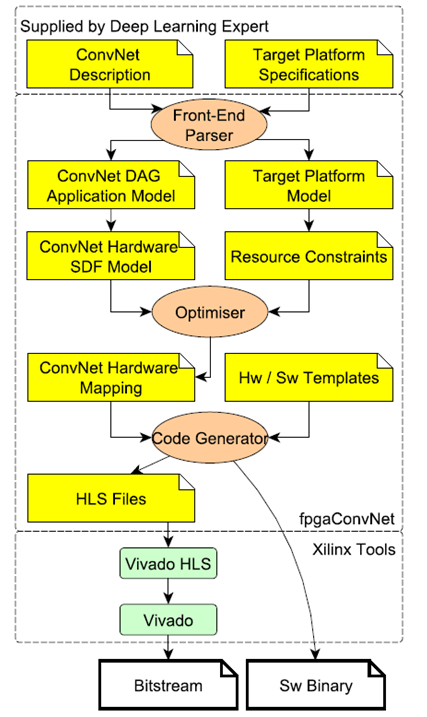
\includegraphics[width=0.4\textwidth]{Figures/fpgaconvnet.png}
%     \caption{fpgaConvNet Architecture. Taken from~\cite{fpgaconvnet}}
%     \label{figure:fpgaconvnet}
% \end{figure}

The fpgaConvNet architecture consists of a Front-End Parser that reads a (ConvNet) description of the network
and a description of the target platform and produces, on the one hand, a
Directed Acyclic Graph (DAG), which is then converted to a Synchronous Data Flow
(SDF) hardware model, and on the other hand, a model of the target platform from
which resource constraints are derived. The hardware model thus obtained goes
into an Optimiser procedure, which produces a hardware mapping. Using hardware
and software templates, a Code Generator procedure generates both the High
Level Synthesis (HLS) input files and the software binaries that will run on the
control CPU embedded in the FPGA. The HLS files go into the Xilinx (FPGA
manufacturer) tools so that the configuration bitstream of the FPGA is produced.


%%%%%%%%%%%%%%%%%%%%%%%%%%%%%%%%%%%%




\section{Darknet Lite}
\label{chapter:Darknet}

As mentioned in Section \ref{sector:DeepVersat}, the DeepVersat system includes a RISC-V CPU to take out generic
code and to write the configuration runs into Versat's memories. This means the first step into implementing software
that can run any convolutional neural network on this system, the software must first run on the CPU then we offload Fixed Functions 
to Versat such as the convolutional layers, max pool, etc.

\subsection{Porting Darknet to an embedded CPU}

As mentioned in Section \ref{section:Darknet} is a framework for Neural Networks on C++ that uses dynamic memory 
and GPU acceleration option to get faster outputs.
Also, the use of floats is prohibited in the embedded code
as the RISC-V CPU only supports the extensions IM. I for Integer and M for multiplication.
It also has a lot of features that are not needed in this work, such as training the CNN.
By stripping the features of Darknet we get a much simpler
code framework appropriately named Darknet lite.

A CNN on Darknet lite is just an array of layers in which each has input, 
output, and layer parameters all defined using a layer struct in which all variables are defined.
Usually, the input is a past layer output or an image input.

% \lstinputlisting[label=DarknetLiteStrut,language=C++,frame=single,breaklines=true,firstline=1,lastline=38,caption=Layer Struct
%   Yolov3~\cite{yolov3}]{./Code/DarknetLiteStrut.h}

By Parsing the .cfg file, a configuration file is written in C with the layer array and static position of the data for each layer. 
Each Layer has its definition in C to be run by the embedded CPU but for the sake of this project, several layers can be
replaced by Functions that utilize Versat, the same way that the original Darknet framework had its functions written for CPU or GPU usage.

% The following figure is an example of a CPU layer that computes the convolutional layer while using Fixed Point Logic.

% \lstinputlisting[label=ConvolutionalLayerCPU,language=C++,frame=single,breaklines=true,firstline=54,lastline=85,caption=Convolutional Layer using only CPU and fixed memory]{./Code/convolutional_layer.c}



\subsection{Parsing CFG Files into the program}

Caffe~\cite{caffe} is a deep learning framework as shown in section \ref{section:toolflow},
using an open source tool~\cite{caffe2darknet}, the output can be set to CFG.
By using the network parser of Darknet, an array of layers is created with all
its required parameters. 

% \lstinputlisting[label=listing:cfg2versat,language=C,frame=single,breaklines=true,firstline=22,lastline=61,caption=For Loop for writing darknet layers ]{./Code/parse2compiler.c}

% Afterward, by going through each layer, "yolo.c" will be written
% with all the data darknet lite will need. 
% In listing \ref{listing:cfg2versat2}, the addresses of the data needed for the layer. 
% In \ref{listing:cfg2versat3}, the static parameters are defined as well.

% \lstinputlisting[label=listing:cfg2versat2,language=C,frame=single,breaklines=true,firstline=15,lastline=21,caption=For Loop for writing darknet layers ]{./Code/yolo.c}

% \lstinputlisting[label=listing:cfg2versat3,language=C,frame=single,breaklines=true,firstline=133,lastline=139,caption=For Loop for writing darknet layers ]{./Code/yolo.c}


%%%%%%%%%%%%%%%%%%%%%%%%%%%%%%%%%%%%%%%%%%%%%%%%%%%%%%%%%%%%%


\section{DeepVersat Software Simulator}
\label{chapter:Simulator}

The need for a software simulator comes from the complexity of the configurations 
being written into Versat and the hardware simulation faults of taking too much time and being hard to debug.

The goal is to emulate what the hardware is doing much more efficiently than 
a simple Hardware simulation as the time of development for hardware
is much higher than for simple software. The Simulator executes clock iteration per iteration 
getting the same results in each clock as the hardware. 
As Versat is a CGRA, different functional unit configurations are easy to accomplish 
in the simulator and the time to get results on performance
for a specific program is a lot faster. 


% The only data the simulator can't output
% is FPGA resource usage the hardware configurations fit the FPGA that is going to be used and the clocks that 
% the hardware can run. But, the propagation time is predictable depending on the number of 
% functional units as the difference between times in different setups are 
% due to the multiplexers on the inputs of the FUs.



\subsection{Architecture and Object Relation}

The Simulator is made up of the Parent Class called Versat, which will be simulated itself, 
as each Versat instance is independent of the others, the simulations are also independent.
The Versat is made up of two CStage Arrays, one is the "live" while the other is the 
shadow registers, where the configurations are held before the simulator is run.
Each Stage is made up of its Functional Units, of which each is connected to the Databus.
As it happens in the hardware, functional units can access the database which has the output 
of the current stage and the previous one.


% \begin{figure}[!htbp]
%     \centering
%     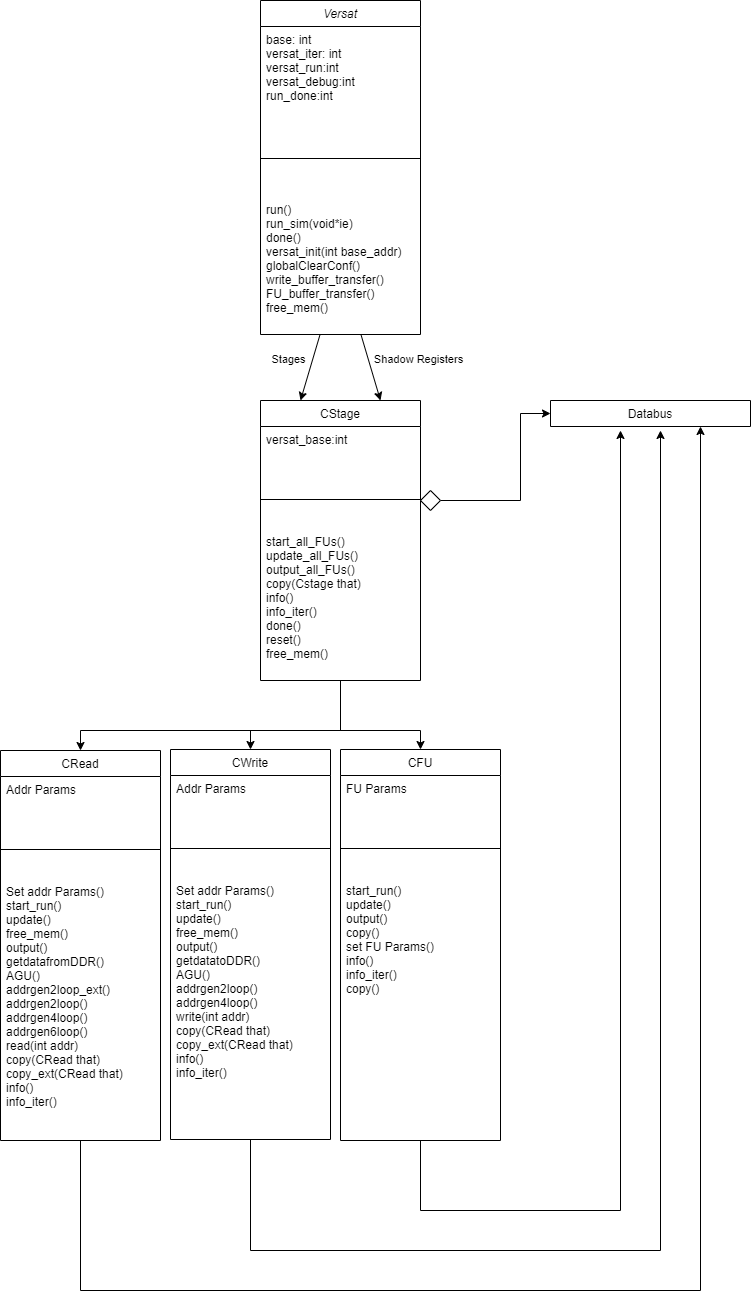
\includegraphics[width=0.4\textwidth]{Figures/VersatSimulatorDraw.drawio.png}
%     \caption{Class Structure for the Versat Simulator}
%     \label{figure:VersatSimulatorClass}
% \end{figure} 


\subsubsection{Functional Units}

The following table contains the functional units present in the simulator. For Memory Units, there are three  FUs possible.CMem, VI and VO.
CMem reads and writes from the databus between CPU and Versat, while VI and VO are made to communicate through DRAM.



\begin{table}[!htbp]
    \centering
    \scalebox{1}{
    \begin{tabular}{|l|l|}
        \hline
        \textbf{Functional Unit}     & \textbf{Porpuse}  \\  \hline
        Read (VI) Mem Unit             & Reads from DDR and \\ & sends Data to databus            \\ \hline
        Write (VO) Mem Unit & Reads from databus \\ & and sends Data to DDR             \\ \hline
        MulAdd (MAC)    & Multiplication and Accumulate          \\ \hline
		Mul    & Multiplication     \\ \hline
		Alu    & Standard algorithmic and \\ & logic unit     \\ \hline
		AluLite    & Stripped down  algorithmic and \\ & logic unit     \\ \hline
		Barrel Shifter (BS) & Shifts to the right or to the left \\ \hline
		Memory (Mem) & Sends/Receives data to/from \\ & the pipeline. Data is inserted through \\ & CPU communication   \\ \hline
        \end{tabular}
    }
    \linebreak
    \caption{Versat Simulator Functional Units}
    \label{table:versatsimfu}
    \end{table}

To add a new FU, it's as easy as creating a new class that will be used by CStage with
a run(), update(), output(), and copy() method. Of course, if it has variables needed to be defined
by the program, set param functions are also needed. Using the simulator, hardware development
and program development can be parallelized to output a new program 
with more optimized performance.

\subsection{Simulation}

After the program that is running on the CPU finishes writing the configurations, it will call the run method of Versat.
In figure \ref{figure:VersatSimulatorSequenceDiagram}, a sequence diagram is presented with the rundown
of a typical program that uses Versat Simulator.


%Previously, a software API was made in a previous thesis~\cite{valter:deepversat}
%for Versat. To build on top of this several, software functions were added to make writing configurations to Versat
%easier.
\begin{figure}[!htbp]
    \centering
    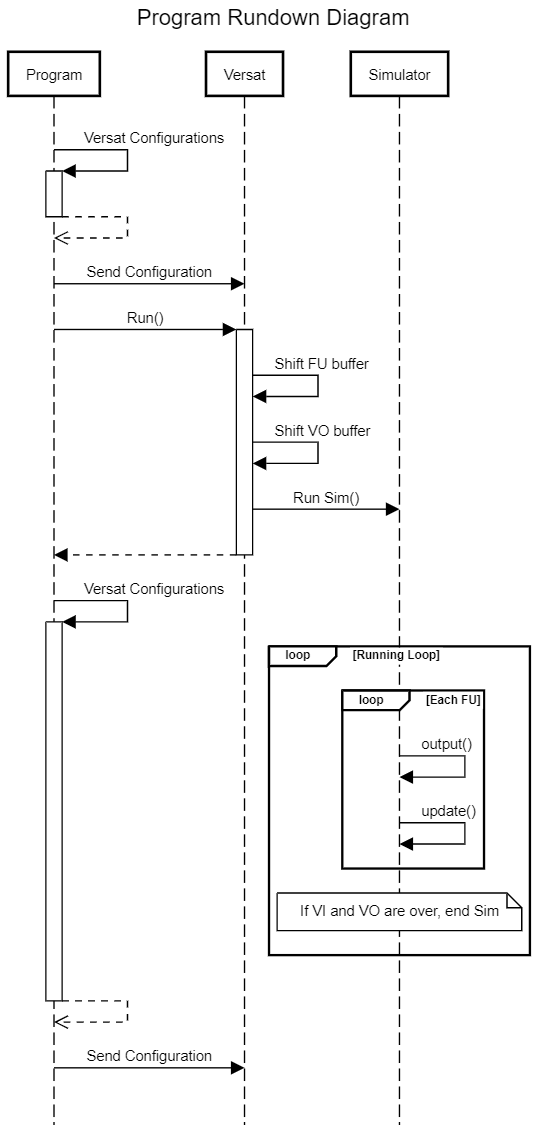
\includegraphics[width=0.4\textwidth]{Figures/versatsim.png}
    \caption{Sequence Diagram of a Program using Versat Simulator}
    \label{figure:VersatSimulatorSequenceDiagram}
\end{figure} 



\subsubsection{Run() Function}

In the software API for Embedded Versat, the run function would write to a shadow register,
which we can call "start" changing the value from zero to 1. 
Similarly, another register would
change the value to 0, which we can call "done". While this last register isn't turned to 1, 
Versat hasn't finished running with the 
previous configurations so all that can be done is to write
configurations for future runs.

In the simulator, it works in a similar way to preserve compatibility 
as the goal is to have the same
programs run on software simulators and the FPGA.

% \lstinputlisting[label=runfunctioncode,language=C++,frame=single,breaklines=true,firstline=222,lastline=245,caption= The Run function code]{./Code/Versat.cpp}

As can be interpreted from~\ref{figure:VersatSimulatorSequenceDiagram}, before running the simulation, there is a reset of the state variables, then shift the 
VO and FU shadow registers.
This is done to simulate the pipeline delay in the FPGA. 
Because the data needs to come and go to the main memory (DDR),
1 run cycle is used just for fetching data and writing data. 
Using a small example:
If a developer writes a configuration to do a 5x5 matrix multiplication, 
Versat will have to run three  times.
Once to fetch data from memory, the second for the actual use of Versat 
and the final one is to get data onto memory.

In the simulator, this is done using the same class instances and 
copying the configuration values. On the hardware, it's several flip-flop registers in a row.
However, all these three  stages can happen at once if you run multiple configurations in one program, 
e.g.: running a CNN
through Versat, will have at least one run per layer. 
So, if it has five layers, Versat will have to run 5+2 times, the last two times are done to
flush the Versat of any data.

After the shift, a new thread is created to run the simulator in parallel 
with the configurations,
having the same behavior as the hardware.

\subsubsection{Start() Method}

At the beginning of the configuration run, the method "start run" of 
all FUs and memories are started.
In this function, several functional units will have their state variables 
reset such as VI,VO and MAC FU.

\subsubsection{Databus}

The databus on Versat is a simple array that holds all the outputs of the functional units.
The data type (versat\_t) of the array depends on the width of Versat, which is part of the configuration file.
Using higher width, e.g: 64 bits, is useful for the same instruction, multiple data (SIMD) 
applications but requires the functional units to be adapted.
For the purpose of this thesis, 16 bits and 32 bits are used depending 
on the neural network and how it is optimized.

When the Versat is instanced in the program, the functional units constructor will point
to the correct position of the databus as it's referenced in the following figure.

As mentioned in figure \ref{figure:deepversatarch} from section \ref{sector:DeepVersat}, 
each functional unit will be able to access the output from the functional units of the
current stage and previous. Software-wise, each stage will be pointing to a part of the databus.  

% INSERT FIGURE HERE


\subsubsection{Update() and Output() Method}


The update method's goal is to update the functional unit's value on the databus. 
Each functional unit has a pipeline delay to output or has a run delay configured, 
like the memories or MAC.

Meanwhile, the output method's goal is to, based on the inputs from the databus, calculate the result from
 the functional Unit.

 For a compute functional unit such as the MAC or the ALU, this means reading from the databus for operands A and B
 and performing the selected operation. For the read memory (VI), it will output an address on the mem
 and performs a read operation. For the write memory, it will output an address and performs a write operation.

%  In the listing \ref{listing:fu}, the code of the Mul functional unit is used as an example.

% \lstinputlisting[label=listing:fu,language=C++,frame=single,breaklines=true,firstline=21,lastline=65,caption=Update and Output method of Mul]{./Code/mul.cpp}


\subsubsection{Copy() and Info() Method}

Finally, the last two functions of the simulator, copy() the main purpose is to copy the configuration parameters from one instance to another,
used mostly at the beginning of the run to simulate the shadow registers.
Meanwhile, the Info method is a State printing function that outputs a string with the full data of the current iteration,
this way, you can check iteration by iteration the progress of the simulation, just like in hardware.
At this moment, if debugging is activated, each clock iteration output and the state of Versat will be in a log file.

% \lstinputlisting[label=listing:fu,language=C++,frame=single,breaklines=true,firstline=572,lastline=584,caption=Info output for the MAC functional unit]{./Code/versat_iter22.txt}


%%%%%%%%%%%%%%%%%%%%%%%%%%%%%%%%%%%%%%%%%%%%%%%%%%%%




\section{Versat API 2.0}
\label{chapter:API}

The Versat API, developed in a previous thesis~\cite{valter:deepversat}, can conceal
the calls to the hardware to avoid changing the program when the hardware changes.

% \lstinputlisting[label=listing:versathpp,language=C++,frame=single,breaklines=true,firstline=17,lastline=40,caption=Sample Versat API implementation for the Hardware for Mem functional unit]{./Code/Versat.hpp}

\subsection{API Architecture}

In figure \ref{newAPI}, a graphic representation of the new API is presented. It has four apparent layers (5 if you count the hardware):

\begin{enumerate}
	\item Complex Mathematical API that is automatically optimized for the Versat Setup you chose. No dev work required
	\item Read/Write using VI and VO for simpler setup of the data. Also includes easier FU functions to set up workloads.
	\item Read/Write configurations for inside Versat Data (Int) or DDR to/from VI/VO (Ext).
	\item Versat API 1.0 where each configuration variable needs to be set up individually
	\item No API. Hardware registers where the values are used inside Versat. 
  \end{enumerate}


\begin{figure}[!htbp]
    \centering
    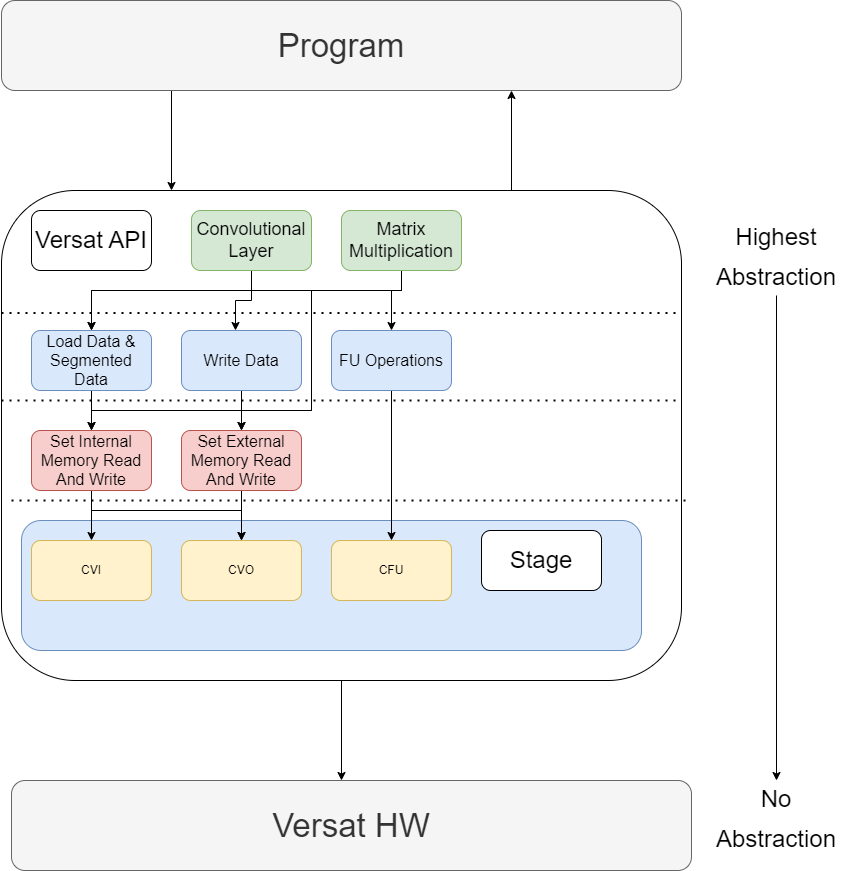
\includegraphics[width=0.4\textwidth]{Figures/VersatMemory.drawio.png}
    \caption{Graphic representation of the new Versat API and its connections}
    \label{newAPI}
\end{figure} 


\subsection{Memory Operations API}

When utilizing the VI instead of a MEM, the data transfer happens between the functional unit and direct memory access while
on the mem, the CPU writes directly to Versat, wasting CPU cycles. For the API, this means going from a read method that is straightforward
to more configuration methods to set up the read operation from DDR The same happens to Write operations. To address this, seven functions were created in two levels of abstraction:
load\_data(),load\_segmented\_data(),write\_data() that use a lower level functions: set\_IntMem\_Write(),set\_ExtMem\_Write(),set\_IntMem\_Read() and set\_ExtMem\_Read().
The function of the higher abstraction memory functions is to abstract the parameters of the AGU. 
% In the following listing, we have one of the implementations
% as an example.

% \lstinputlisting[label=listing:loadsegdata,language=C++,frame=single,breaklines=true,firstline=366,lastline=376,caption=Load Segmented Data code]{./Code/versat_configurations.cpp}


Although this means having to write code with the AGUs in mind
and how they function. To avoid it, a new class was created to also abstract how the AGU counts loops and approximate 
the code to simple C++ code that runs on a CPU.

% \lstinputlisting[label=listing:accumulator,language=C++,frame=single,breaklines=true,firstline=72,lastline=110,caption=Accumulator Class code]{./Code/versatnew.hpp}

To transform from AGU parameters to for loop, it depends on the number of loops pretended to be done. VI AGU is three  cascade Accumulators
and as such, the increment on the second and third accumulators needs to be adjusted.

% \lstinputlisting[label=listing:intmemread,language=C++,frame=single,breaklines=true,firstline=77,lastline=86,caption=AGU parameters to Simple forloop parameters transform]{./Code/versat_configurations.cpp}

\subsection{Matrix Multiplication and Dot Product}

As part of the new API, a matrix multiplication function was added. To implement this function, first, two Accumulator class variables are initialized.
Afterward, using the two arrays address in DDR, the AGU configurations of the VIs to read from the main memory are set, then the AGU configurations of VI for the data handling inside the Data Engine.
Finally, the function that will write the configuration of a MAC and the store AGU configurations. This last step is optional as the result of this matrix multiplication can be used in the same run
to make other operations e.g.: adding a bias using one of the ALUs to the results.

% \lstinputlisting[label=listing:matrixmult,language=C++,frame=single,breaklines=true,firstline=167,lastline=215,caption=Matrix Multiplication Configurations]{./Code/versat_configurations.cpp}

The Dot product function is very similar, the configurations are identical for the data transfer from the main memory to the VIs. In the inside loops of the VIs, instead of three  loops, we only need to use 
1.

\subsection{Generic Convolution}

As explained previously, convolutional neural networks are a type of neural nets that are 
used mostly in image and object recognition by using convolutional layers. To run a convolutional layer on Versat with
optimized performance, the configurations must be written with regard to several parameters:

\begin{enumerate}
	\item Memory Sizes used in VI and VO. The amount of data that can be stored at once. It determines the number of outputs done per run.
	\item Functional Units used in the Data Engine. Here it's about the lowest common denominator, i.e. the bottleneck in the Data Engine determines the number of outputs done simultaneously.
  \end{enumerate}
 
This function has a total of 20 variables calculated at the start before the Versat configurations are written. The most important
variables are the following:

\begin{itemize}
	\item output height (h) and width (w) of the resulting matrix from the convolution.
	\item Number of outputs done simultaneously, also known as pipeline width (nOutputs). This value is pre-compiled as it depends on only Versat Configurations.
	\item Number of outputs that can be done per VI (y) in a single run and its variations. Outputs total (y\textsubscript{2}), Output Lines per VI (y\textsubscript{3}) Output Lines total (y\textsubscript{4}).
The value of y4 and y2 decide the different configuration scenarios.
	\item Resource Allocation Variables
which are explained in subsection \ref{ConvolutionScenarios}
	\item Address Variables
	\item AGU Configuration Variables
  \end{itemize}

The hard part of the algorithm is to allocate the data in the most efficient way possible and to create the AGU configurations
for the VIs and VOs. For this algorithm, the CGRA will act like a GPU pipeline where several "threads" will exist
that will output one point every k\textsuperscript{2} cycles, where k is the kernel size used in the convolution.

\begin{figure}[!htbp]
    \centering
    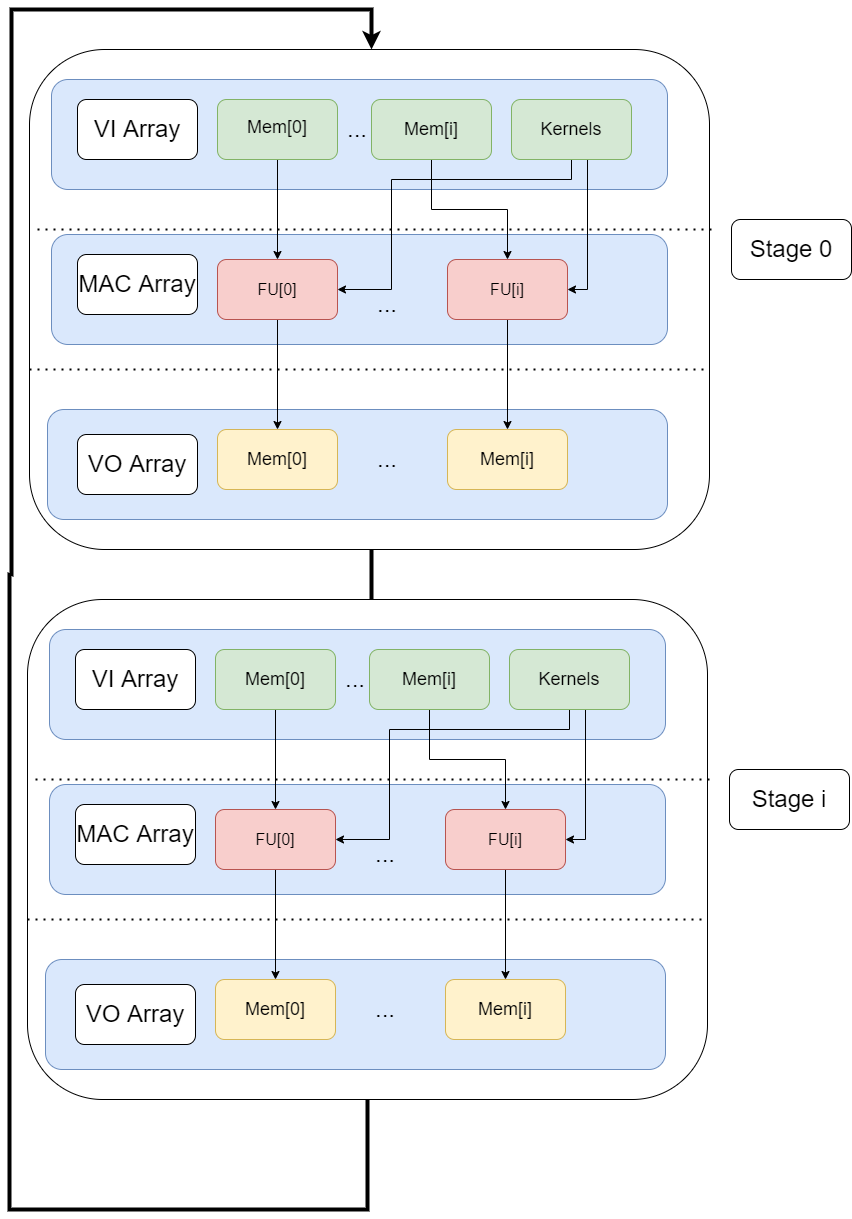
\includegraphics[width=0.4\textwidth]{Figures/Convolution.drawio.png}
    \caption{Versat Configuration goal in Graphical form}
    \label{VersatConfiguration}
\end{figure}

\subsubsection{Loading Data}

Usually, when doing a convolution in CPU, the frameworks transform the convolution to a matrix multiplication by creating a new matrix that will multiply with a
kernel vector. It's done this way as matrix multiply is a heavily optimized operation and can take advantage of a CPU's SIMD units or even call the GPU APIs
and offset the workload there. On Versat, this is not needed as to calculate one output, we will need only enough space in mem to hold
k\textsuperscript{2}*ch where ch is the channels of the input. And as such, it means 9216 bytes per VI at least for YoloV3 CNN when using 16-bit operands.

To load the data onto the mems in Versat, we will load segmented data. That is, for each mem, we will load the data
needed to do y iterations or y\textsubscript{3} iterations, depending on which convolution scenario it is.
The more inputs are transferred to a VI mem, the more efficient it is as data doesn't need to be replicated as much between the instances,
i.e. for the first output, there's a need for k\textsuperscript{2}*ch inputs, but for other sequential outputs, if the stride is one only k*ch more inputs are needed.
of course, this is only true if the stride is lower than the kernel size.

On the code, this takes form in one single line, thus the importance of the previously written functions.

\lstinputlisting[label=listing:memread,language=C++,frame=single,breaklines=true,firstline=446,lastline=446,caption=Load Input Matrix into VIs]{./Code/versat_configurations.cpp}

where the variable "size per channel" can be calculated with the following formula:

\[ size=w*(k+stride*(iter-1)) \]

where w is the width of the input matrix, k is the kernel size and iter is the number of iterations that this mem will run.

\subsubsection{Convolution Scenarios}
\label{ConvolutionScenarios}

\begin{figure}[!htbp]
    \centering
    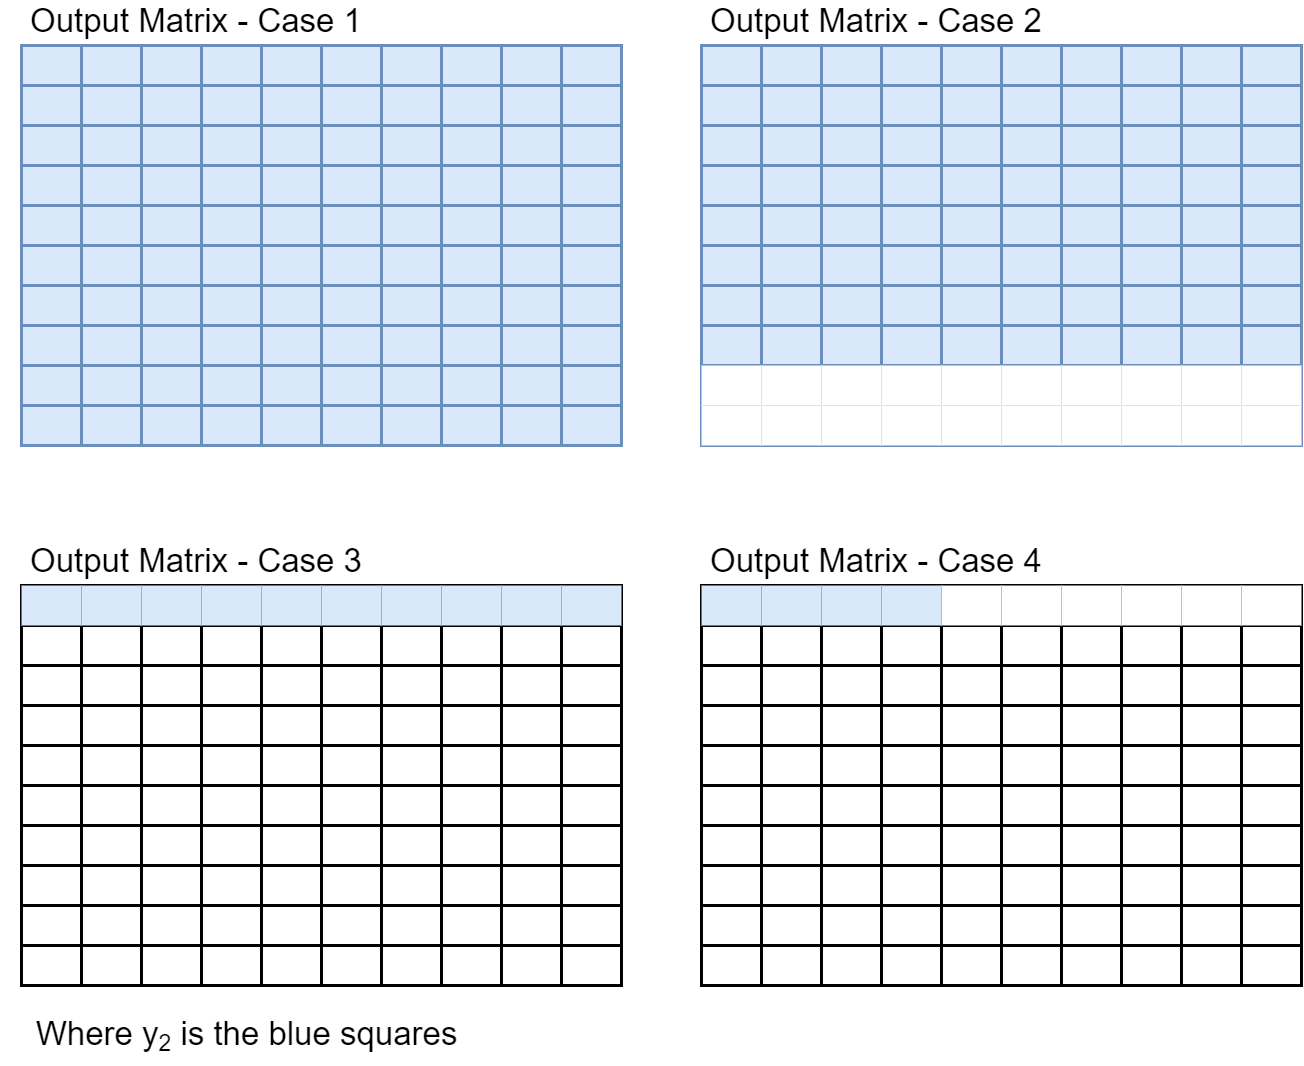
\includegraphics[width=0.4\textwidth]{Figures/Variables.drawio.png}
    \caption{Convolution Scenarios that Versat will have}
    \label{ConvScenarioss}
\end{figure}

When writing the configurations of the convolution runs, there are several cases the software needs to take into consideration.
As explained in the previous subsection, the data that the VIs can handle and the number of datapaths that the data can have influenced
the convolution scenarios. For this function, four were implemented and are presented in figure \ref{ConvScenarioss}.


The different hardware configurations and the endless possibilities for convolutions mean that all possibilities are covered. 
The only limitation of this generic function is to make partial results which is the last possible case where the mem can't handle enough inputs for 
1 output.


% \begin{figure}[!htbp]
%     \centering
%     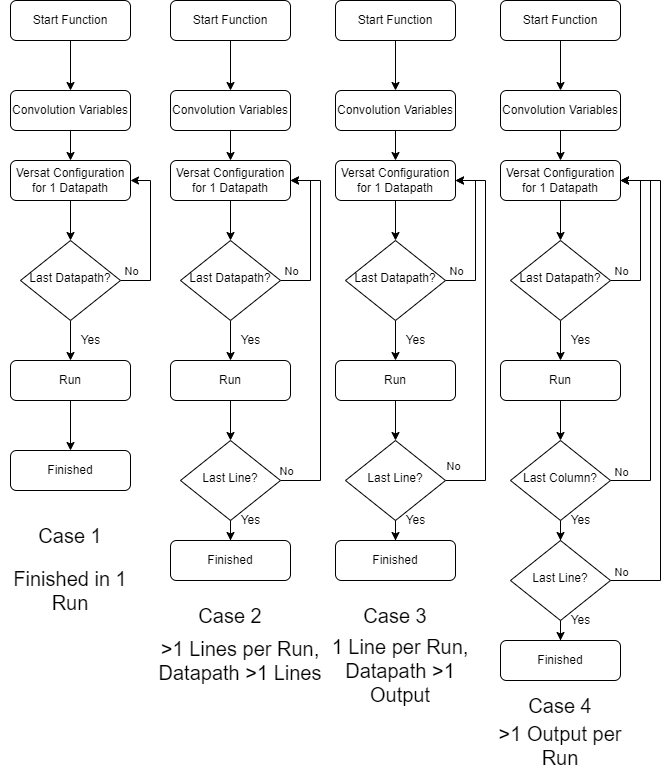
\includegraphics[width=0.4\textwidth]{Figures/ConvolutionFlowChart.drawio.png}
%     \caption{Configuration Flowchart for the different scenarios}
%     \label{ConvFlowChart}
% \end{figure} 

% And on listing \ref{listing:convfinal} the AGU configurations of the VIs that hold the input matrix, the MAC configuration, and finally
% the VO AGU configuration.

% \lstinputlisting[label=listing:convfinal,language=C++,frame=single,breaklines=true,firstline=449,lastline=478,caption=Versat configurations for one datapath]{./Code/versat_configurations.cpp}


%%%%%%%%%%%%%%%%%%%%%%%%%%%%%%%%%%%%%%%%%%%%%%%%%%%%%%%%%%%%%%%%%%%


\section{Results}
\label{chapter:results}

%%%%%%%%%%%%%%%%%%%%%%%%%%%%%%%%%%%%%%%%%%%%%%%%%%%%%%%%%%%%%%%%%%%%%%%%
\subsection{Simulator Testing}
\label{section:simtest}

To test the simulator, a testbench was created that will create a random input matrix of 5x5
with a kernel size of 3. For each Stage defined in the headers file, a channel will be added and
the result of the convolution will propagate through the stages.

To be more specific in the beginning, the configurations of the VIs are written to transfer the data
from the program to Versat. The data uses the rand() function with seed using current time
so the result is different every time. Both the input matrix and kernel map are randomized.
The former value varies from -25 to 25 while the kernel varies from -5 to 5. Using the data, 
we calculate the result of the convolution in the CPU. Afterward, the configuration for the Bias mem
is done and then stage by stage the configuration of the VI, MAC, and ALU is done. Finally, the
configuration of the VO is written.

% \begin{figure}[!htbp]
%     \centering
%     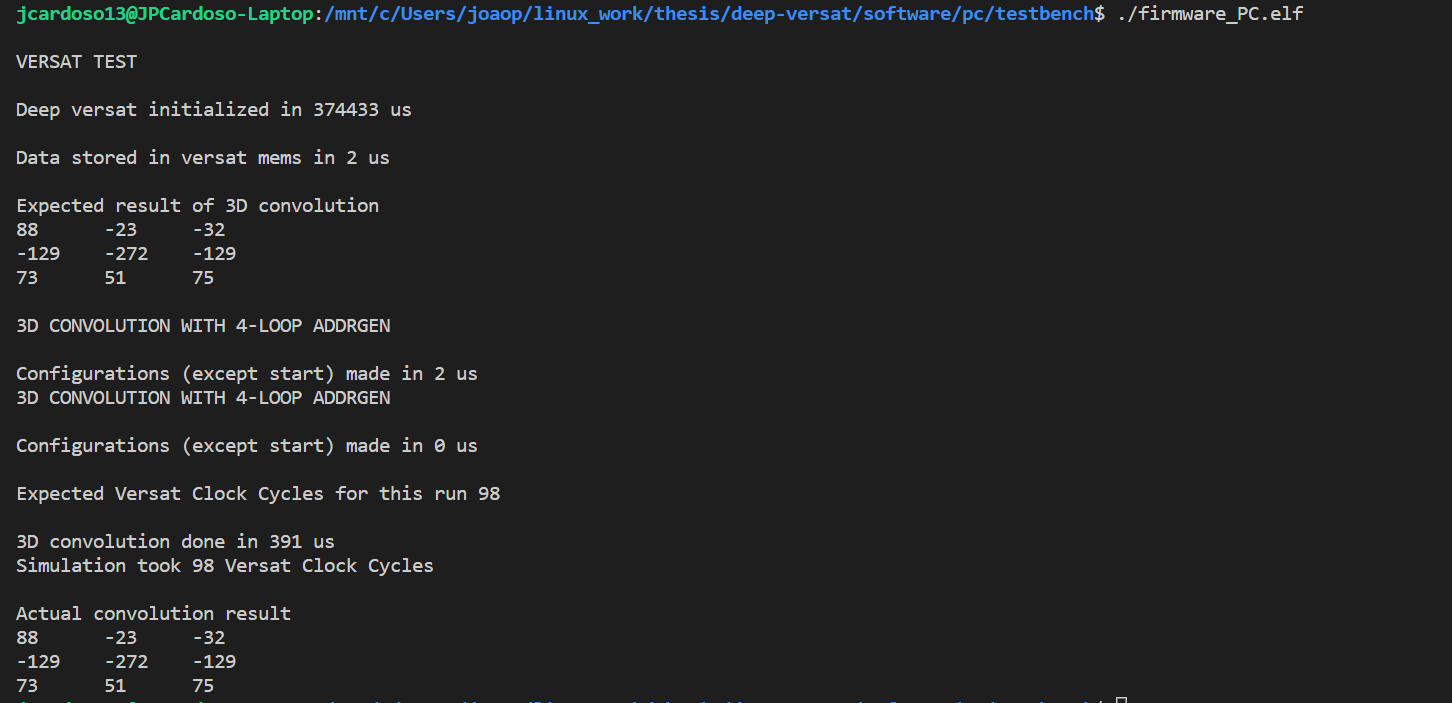
\includegraphics[width=0.4\textwidth]{Figures/test1.png}
%     \caption{Simulator test output in terminal}
%     \label{figure:test1}
% \end{figure} 

The estimated iterations needed are the following:

\[ Est=Delay+Iter_2*Per_2*Iter_1*Per_1\]

Where these are the AGU configurations of the VO where the results are written. The Delay is accumulated
through the several stages by adding two due to the MACs and ALUs.

%%%%%%%%%%%%%%%%%%%%%%%%%%%%%%%%%%%%%%%%%%%%%%%%%%%%%%%%%%%%%%%%%%%%%%%%
\subsection{Testing the new API}
\label{section:testgencov}

In this section, the same method for the previous testbench is made. 
While the previous one relies on using API v1 for the configuration, these test benches
run the new API. 

\subsubsection{Testbench for Matrix Multiplication}

The Matrix Multiplication is a quite simple program. The only thing needed is an instance
Versat, run versat\_init(), create the matrixes, and then use the function matrix\_multiplication()
The data is also computed in the CPU the result to verify the output.

% \begin{figure}[!htbp]
%     \centering
%     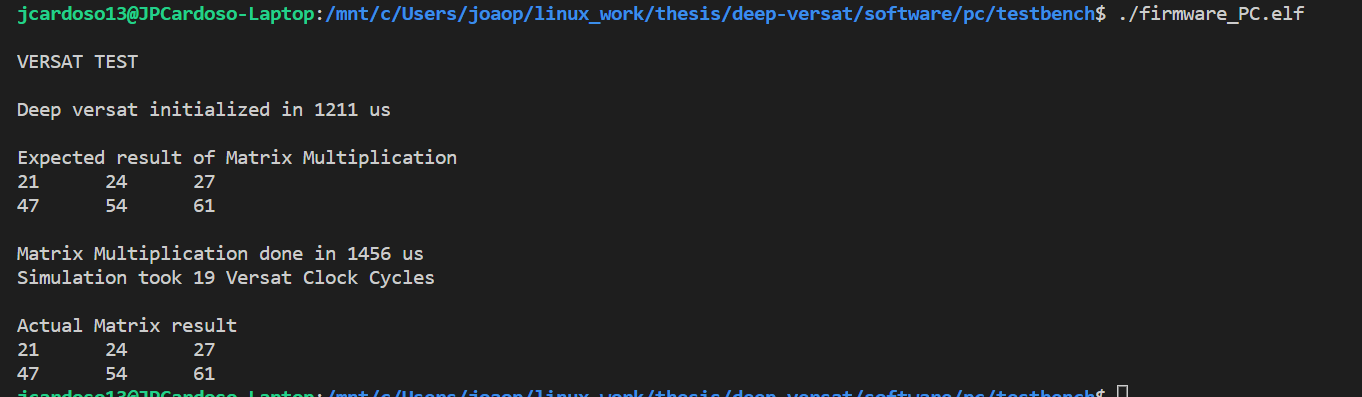
\includegraphics[width=0.4\textwidth]{Figures/test2.png}
%     \caption{Matrix Multiplication Testbench Outputs}
%     \label{figure:test2}
% \end{figure}

\subsubsection{Testbench for Generic Convolution}

Using the same method on the previous test benches, the following Convolution Layer was used
with several Versat Configurations.

\begin{table}[!htpb]
    \centering
    \begin{tabular}{ll}
    \hline
    \textbf{CNN Variable} & \textbf{Value}        \\ \hline
    Kernel Size            & 2                 \\
    Channels            & 2                       \\
    Number of Kernels            & 2                       \\
    Input Height                  & 12                        \\
    Input Width                & 12                  \\
    Stride              & 1                     \\
    Out Width               & 11                      \\
    Out Height            & 11  \\
    Out Channels                   & 2                     \\ \hline
    \end{tabular}
    \label{table:convInput}
    \linebreak
    \caption{CNN Layer on the testbench}
\end{table}

% With this layer, figure \ref{figure:test3} has the output result of the generic convolution testbench.

% \begin{figure}[!htbp]
%     \centering
%     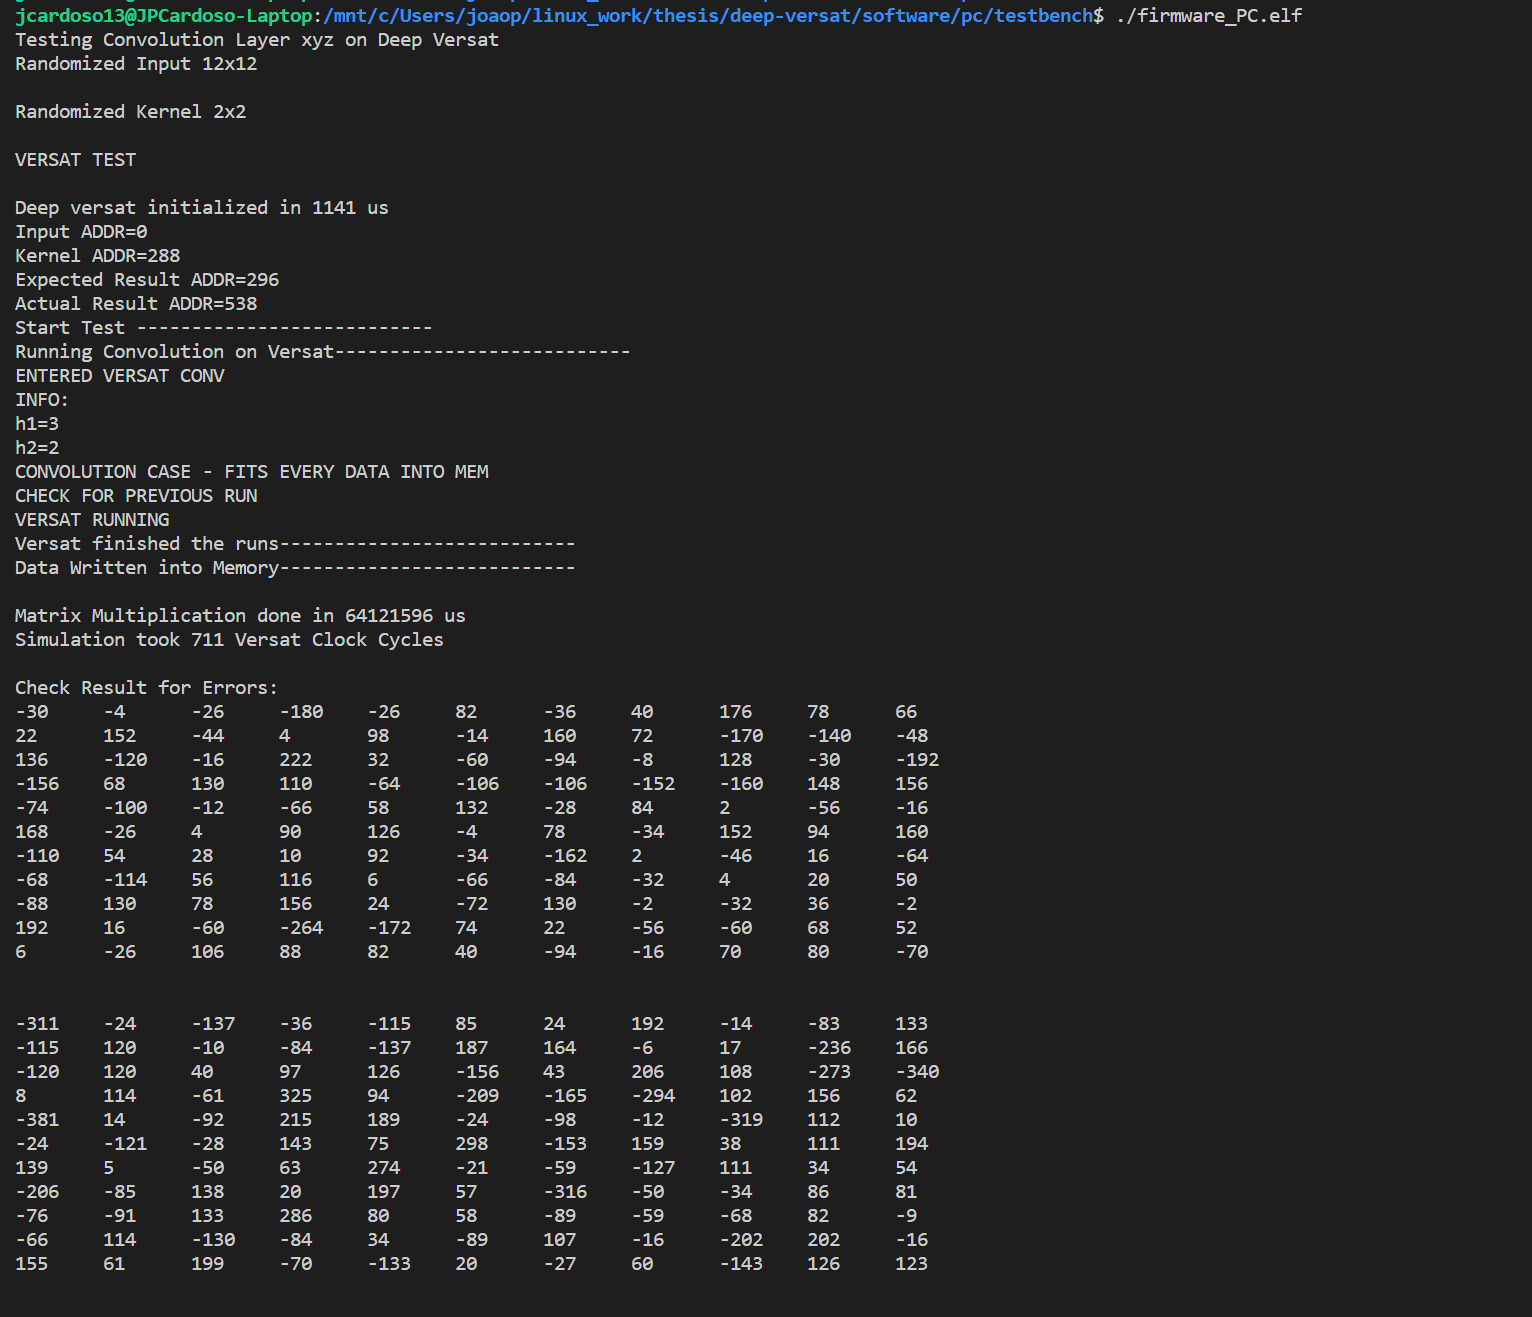
\includegraphics[width=0.4\textwidth]{Figures/test3.png}
%     \caption{Generic Convolution Testbench Outputs}
%     \label{figure:test3}
% \end{figure}

In Table \ref{table:Iterations}, the different Datapath numbers and how it affects performance.
A datapath is a combination of one VI, one MAC, and one VO. So the lower number in the Versat configuration file
decides the number of valid datapaths, of course, VI needs +1 in numbers more than the functional units due to the Kernel memory.

\begin{table}[!htpb]
    \centering
    \begin{tabular}{ll}
    \hline
    \textbf{Number of Datapaths} &  \textbf{Iterations}        \\ \hline
    1          & 1943                 \\
	2          & 1063                 \\
	3          & 711                 \\
	4          & 535                 \\
	6          & 359                 \\
	8          & 359                 \\
	11          & 183                 \\
	16          & 183                 \\
    22            & 183                       \\  \hline
    \end{tabular}
    \label{table:Iterations}
    \linebreak
    \caption{CNN Layer on the testbench with several Versat hardware configurations}
\end{table}

The reason for these results is quite simple. In total, 11 output lines are divided
by the datapaths. When the division is not a whole number, the remainder gets distributed
by available datapaths. The consequence of this, when changing from six to eight datapaths, the performance
doesn't get any better. Datapath zero will have to run twice to (2 lines) while Datapath eight will run one line.
To increase further the performance, the output channels would have to be divided through more datapaths.

% The tests were executed on a 64-bit machine, with an AMD Ryzen 7 5800H Processor and 16GB of RAM running
% Windows 11, version 22H2, WSL 2.0 with the image of Ubuntu 20.04. The compiler used is g++ version 9.4.0.


%%%%%%%%%%%%%%%%%%%%%


\section{Conclusions}
\label{chapter:conclusions}

In this paper, several modules and tools were presented for neural networking development on Versat.
The simulator is a significant improvement over normal hardware simulation for testing new
software configurations and workloads. It also can predict the performance of the workloads
and helps size how many functional units, stages, or how much the size of memories should be
to achieve the highest performance.
Furthermore, the new Versat API can bring new tools for development using the hardware
and be able to write code for Versat akin to writing normal C++ code that runs on a CPU.
Finally, the tools designed for Darknet give embedded development a boost by being able to
run any CNN on embedded hardware, even if it's just a CPU.
To test this, a suite of programs was planned and the results show the new software tools
effectiveness.

% ----------------------------------------------------------------------
\subsection{Achievements}
\label{section:achievements}

One achievement of this paper was the development of the simulator. The simulator is able
to successfully emulate the output of the hardware, where a new program written for Versat
can be tested in five seconds instead of several minutes to put the program into the FPGA.
Another achievement is the generic convolution being able to run any type of convolution layer
efficiently. By changing the Versat parameters, a new complete hardware configuration can be
done and tested with the software to check new performance figures.
Lastly, the darknet framework for embedded devices and the tools used to parse CFG
are important for future work using the Versat CGRA.





%%%%%%%%%%%%%%%%%%%%%%%%%%%%%%%%%%%%%%%%%%%%%%%%%%%%%%%%%%%%%%%%%%%%%%%%%%%%%%%%%%%%%%%%%%%
% \lstset{language=C++}
% \lstset{basicstyle=\scriptsize}
% \begin{figure}[!htb]
% \begin{minipage}{\linewidth}
% \begin{lstlisting}[frame=single]
% #include "Vsystem.h"
% #include "verilated.h"
% #include "verilated_vcd_c.h"

% vluint64_t main_time = 0; 
% double sc_time_stamp () {
% 	return main_time;
% }

% int main(int argc, char **argv, char **env)
% {
% 	Verilated::commandArgs(argc, argv);
% 	Verilated::traceEverOn(true);
% 	Vsystem* top = new Vsystem;
% 	VerilatedVcdC* tfp = new VerilatedVcdC;
% 	top->trace (tfp, 99);
% 	tfp->open ("waves.vcd");
	
% 	top->clk = 0;
% 	top->databus_sel = 0;
% 	top->databus_rnw = 1;
% 	top->databus_addr = 0;
% 	top->databus_data_in = 1;
	
% 	int t = 0;
	
% 	while (!Verilated::gotFinish()) {
% 		if (t > 200)
% 			top->resetn = 1;
% 		top->clk = !top->clk; //Toggle clock
% 		top->eval();          //Evaluate the model
% 		tfp->dump (t);        //Write to VCD file
% 		t += 5;               //Increment clock
% 		if (top->resetn && top->trap == 1)
% 			Verilated::gotFinish(true);
% 	}

% 	tfp->close(); //Close the VCD
% 	top->final(); //Finish the simulation
% 	delete top;
% 	exit(0);
% }
% \end{lstlisting}
% \end{minipage}

% 	\caption{Example testbench in C++ for RV32-Versat}
% 	\label{fig:tb_cpp}
% \end{figure}
% \lstset{basicstyle=\normalsize}


%%%%%%%%%%%%%%%%%%%%%%%%%%%%%%%%%%%%%%%%%%%%%%%%%%%%%%%%%%%%%%%%%%%%%%%%%%%%%%%%%%%%%%%%%%

% \begin{figure}[!htb]
% 	\centering
% 	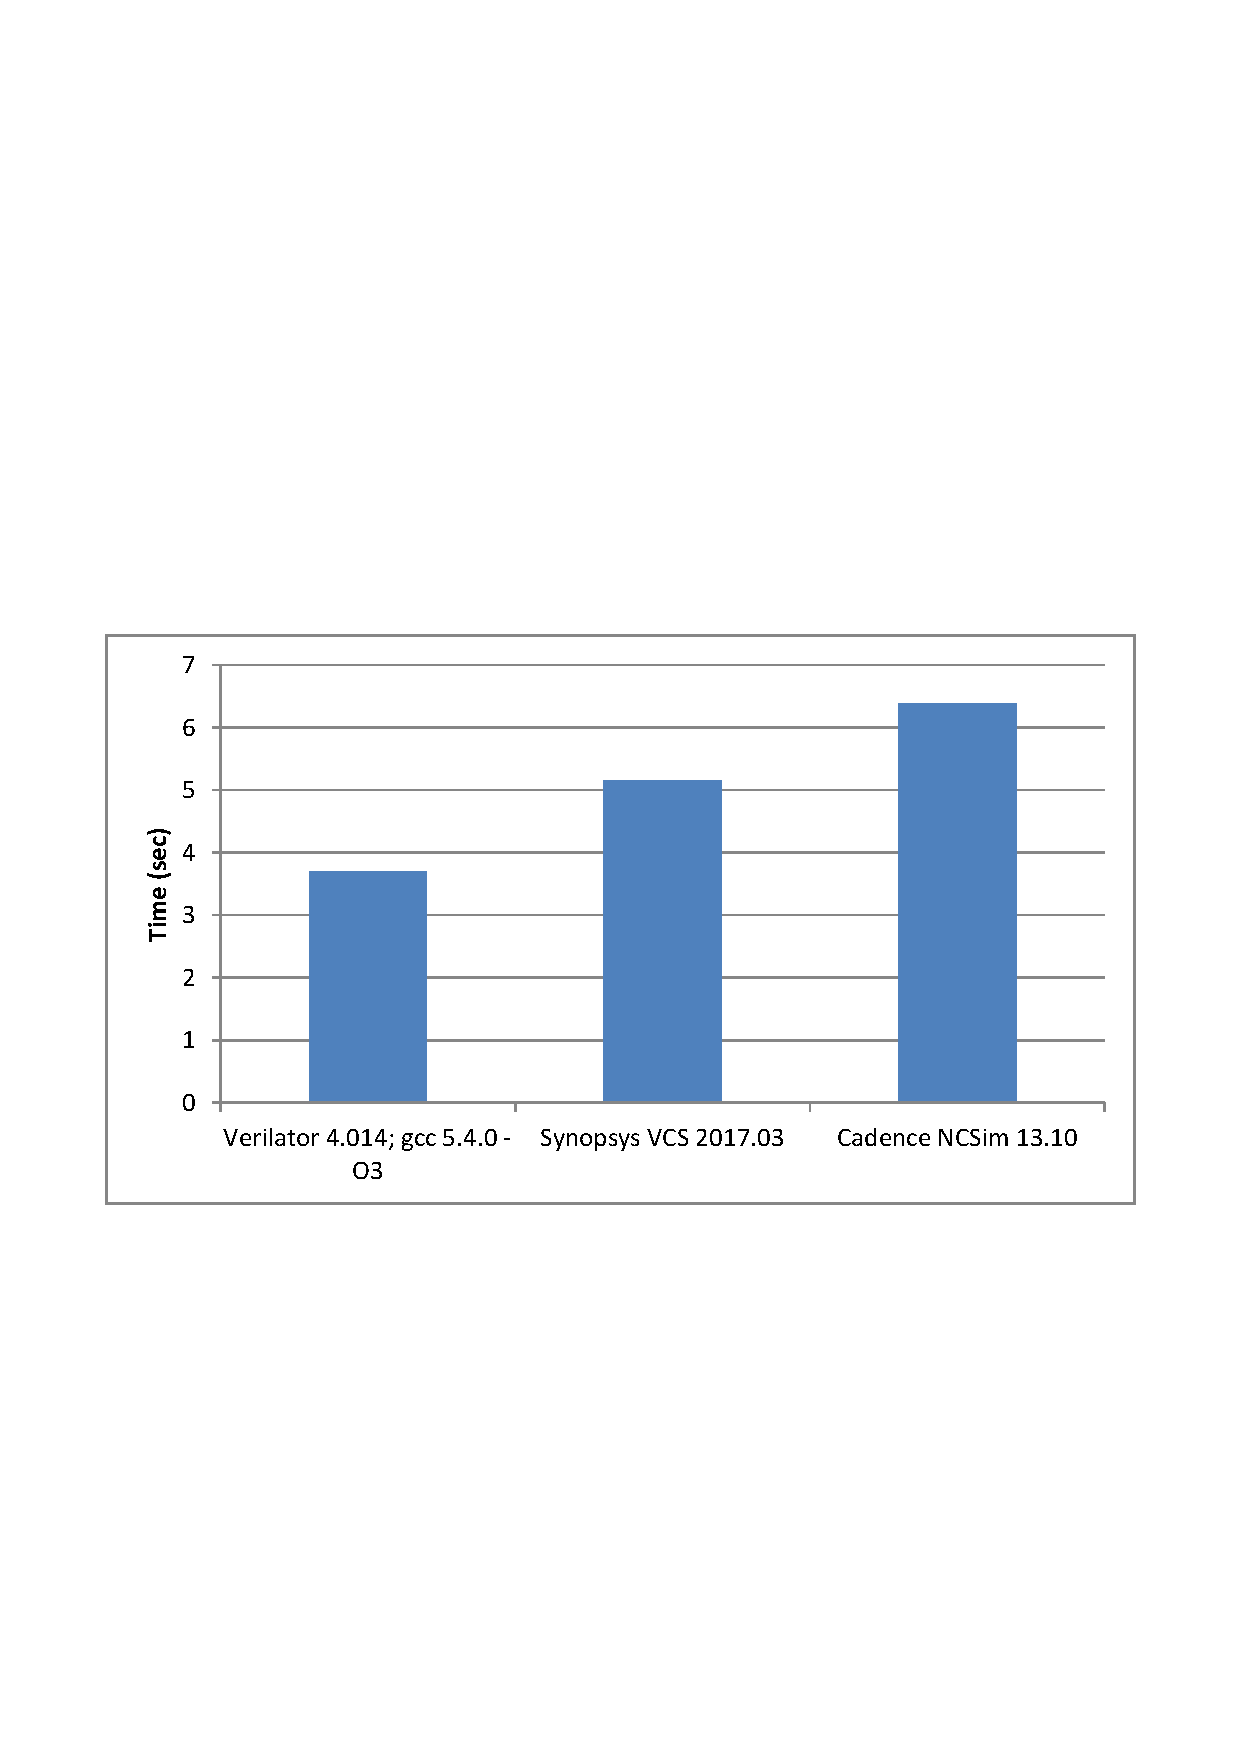
\includegraphics[trim=0 250 0 290 , clip, width=0.4\textwidth]{Figures2/benchmark.pdf}
% 	\caption{Benchmark results for RV32-Versat running the convolutional neural network.}
% 	\label{fig:benchmark}
% \end{figure}

% \begin{figure}[!htb]
% 	\centering
% 	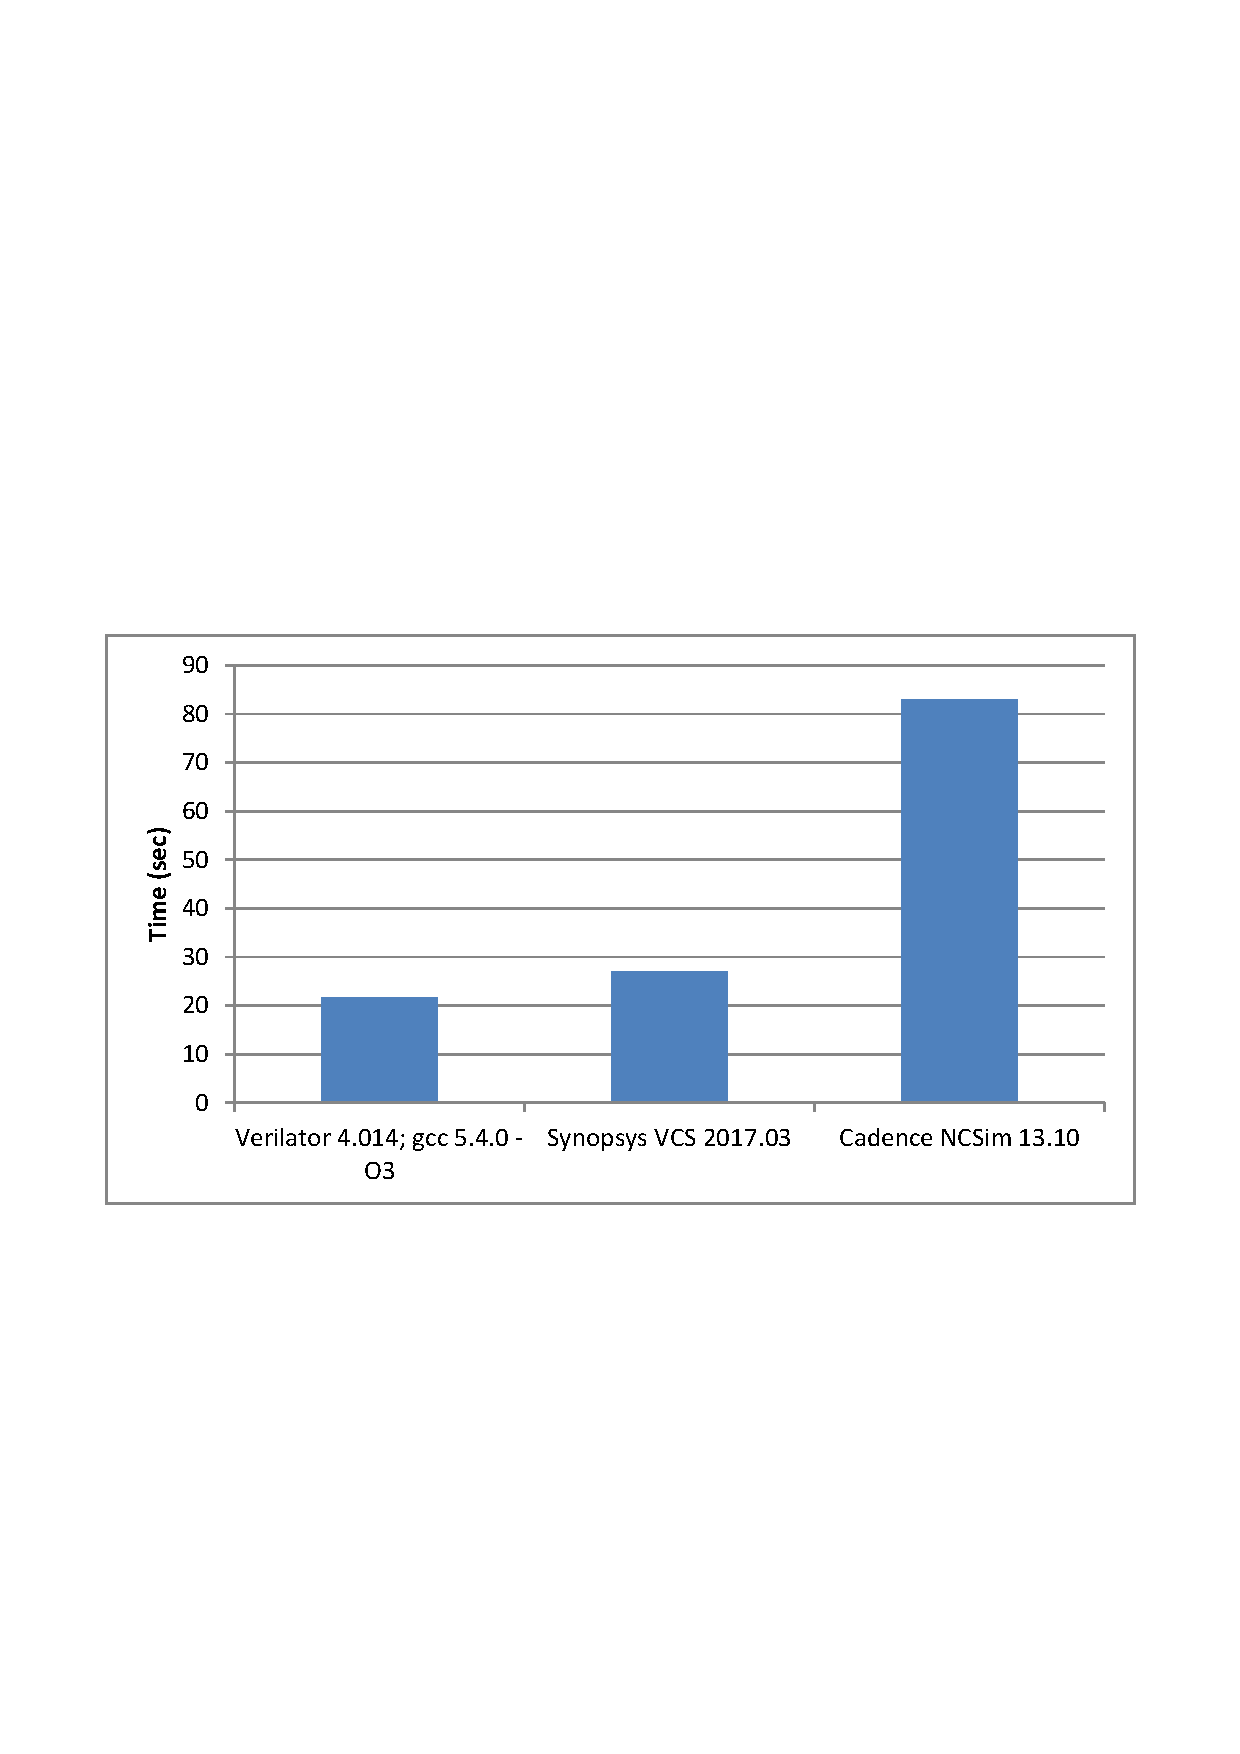
\includegraphics[trim=0 250 0 290 , clip, 
% 	width=0.4\textwidth]{Figures2/benchmark_vcd.pdf}
% 	\caption{Benchmark results for RV32-Versat running the convolutional neural network. 
% 		Debug mode and
% 		vcd generation enabled.}
% 	\label{fig:benchmark_vcd}
% \end{figure}


%\section*{Acknowledgment}

%The preferred spelling of the word ``acknowledgment'' in America is without 
%an ``e'' after the ``g''. Avoid the stilted expression ``one of us (R. B. 
%G.) thanks $\ldots$''. Instead, try ``R. B. G. thanks$\ldots$''. Put sponsor 
%acknowledgments in the unnumbered footnote on the first page.

\bibliographystyle{unsrt}
% argument is your BibTeX string definitions and bibliography database(s)
\bibliography{Thesis_bib_DB}

\end{document}
